Besides linear cryptanalysis, differential cryptanalysis is probably the most established cryptanalytic method against block ciphers~\cite{des-dc}. In this chapter we combine algebraic techniques with differential cryptanalysis to various novel algorithms. We also show the viability of our new methods by applying them to reduced variants of the block ciphers \PRESENT and KTANTAN32.

This chapter consists of a revised, updated and extended version of the paper titled ``Algebraic Techniques in Differential Cryptanalysis'' by Carlos Cid and the author presented at FSE 2009 \cite{adc:fse2009}. Some results were also published in the paper ``Algebraic Precomputations in Differential and Integral Cryptanalysis'' by Carlos Cid, Thomas Dullien, Jean-Charles Faugère, Ludovic Perret and the author \cite{acdfp:inscrypt2010}. Furthermore, some results in this chapter were also presented at the Tools for Cryptanalysis 2010 workshop. The experimental results against KTANTAN32 are unpublished but were partly presented at the rump session of the Early Symmetric Cryptography Seminar 2010 in Remich, Luxembourg. The later results were obtained while visiting the group of Jean-Charles Faugère in Paris in 2009.

This chapter is structured as follows. First, we briefly describe differential cryptanalysis and give the basic idea of the attack in Section~\ref{sec:overview}. We then describe the block cipher \PRESENT in Section~\ref{sec:present} and existing attacks against a reduced round versions of \PRESENT. In Section~\ref{sec:ktantan32} we describe the block cipher KTANTAN32. In Section~\ref{sec:adc} we describe the application of our new attack technique against reduced round versions of \PRESENT and KTANTAN32. We present a brief discussion of the attacks and possible extensions in Section~\ref{sec:discussion}.


\section{Overview of the New Attack Technique}
\label{sec:overview}
Since our approach combines differential and algebraic cryptanalysis, we briefly describe differential cryptanalysis below. Algebraic cryptanalysis was discussed in Chapter~\ref{chapter:algebraic_attacks}.

\subsection{Differential Cryptanalysis}
Differential cryptanalysis was formally introduced by Biham and Shamir at Crypto'90 \cite{Biham1991}, and has since been successfully used to attack a
wide range of block ciphers. In its basic form, the attack can be used to distinguish a $n$-bit block cipher from a random permutation. By considering the distribution of output \emph{differences} for the non-linear components of the cipher (e.g. the S-Box), the attacker may be able to construct \emph{differential characteristics} \mbox{$P' \oplus P'' = \Delta P \rightarrow \Delta C = C' \oplus C''$} for a number of rounds $N$ that are valid with probability $p$. If $p \gg 2^{-n}$, then by querying the cipher with a large number of plaintext pairs with prescribed difference $\Delta P$, the attacker may be able to distinguish the cipher by counting the number of pairs with the output difference predicted by the characteristic. A pair for which the characteristic holds is called a \emph{right pair}. A pair which is not a right pair is a \emph{wrong pair}.

By modifying the attack, one can use it to recover key information. Instead of characteristics for the full $N$-round cipher, the attacker considers characteristics valid for $r$ rounds only ($r = N - R $, with $R>0$). If such characteristics exist with non-negligible probability the attacker can guess some key bits of the last rounds, partially decrypt the known ciphertexts, and verify if the result matches the one predicted by the characteristic. Candidate (last round) keys are counted, and as random noise is expected for wrong key guesses, eventually a peak may be observed in the candidate key counters, pointing to the correct round key\footnote{In some variants, as described in \cite{fulldes-dc}, no candidate key counters are required; see Section~\ref{sec:discussion} for a brief discussion of this attack.}.

Note that due to its statistical nature, differential cryptanalysis requires a very large number of plaintext-ciphertext pairs (for instance, approximately $2^{47}$ chosen plaintext pairs are required to break DES \cite{fulldes-dc}). Many extensions and variants of differential cryptanalysis exist, such as the Boo\-merang attack \cite{Wagner1999} and truncated and higher-order differentials \cite{Knudsen1995}. The technique is however very well understood, and most modern ciphers are designed to resist to differential cryptanalysis. This is often achieved by carefully selecting the cipher's non-linear operations and diffusion layer to make sure that if such differential characteristics exist, then $r \ll N$ which ensures that backward key guessing is impractical. The AES is a prime example of this approach~\cite{Daemen2002}.

\subsection{Algebraic Techniques in Differential Cryptanalysis}

A first idea in extending algebraic cryptanalysis is to use more plain\-text--cipher\-text pairs to construct the equation system. Given two equation systems $F'$ and $F''$ for two plaintext--ciphertext pairs $(P',C')$ and $(P'',C'')$ under the same encryption key $K$, we can combine these equation systems to form a system $F = F' \cup F''$. Note that while $F'$ and $F''$ share the key and key schedule variables, they do not share most of the state variables. Thus the cryptanalyst gathers almost twice as many equations, involving however many new variables. Experimental evidence indicates that this technique may often help in solving a system of equations at least up to a certain number of rounds~\cite{faugere:fse2007,bulgin-brickenstein:eprint2008}. The second step is to consider probabilistic relations that may arise from differential cryptanalysis, giving rise to what we call \emph{Attack-A}.

\subsubsection{\emph{Attack-A}.}

For the sake of simplicity, we assume the cipher is an Substitution-Permutation-Network (SP-net\-work), which iterates layers of non-linear transformations (e.g. S-Box operations) and affine transformations. Now consider a differential characteristic $\Delta = (\delta_0, \delta_1, \ldots , \delta_r)$ for a number of rounds, where $\delta_{i-1} \rightarrow \delta_{i}$ is a one-round difference arising from round $i$ and valid with probability $p_{i}$. If we assume statistical independence of one-round differences, the characteristic $\Delta$ is valid with probability $p = \prod p_i$. Each one-round difference gives rise to equations relating the input and output pairs for active S-Boxes. Let $X'_{i,j}$ and $X''_{i,j}$ denote the $j$-th bit of the input to the S-Box layer in round $i$ for the systems $F'$ and $F''$, respectively. Similarly, let $Y'_{i,j}$ and $Y''_{i,j}$ denote the corresponding output bits. Then we have that the expressions
$$
X'_{i,j} + X''_{i,j} = \Delta X_{i,j} \rightarrow \Delta Y_{i,j} = Y'_{i,j} + Y''_{i,j},
$$
where $\Delta X_{i,j}, \Delta Y_{i,j}$ are known values predicted by the characteristic, are valid with some non-neg\-ligible probability $q$ for bits of active S-Boxes. Similarly, for non-active S-Boxes (that are not involved in the characteristic $\Delta$ and therefore have input/output difference zero), we have the relations
$$
X'_{i,j} + X''_{i,j} = 0 = Y'_{i,j} + Y''_{i,j}
$$
also valid with a non-negligible probability.

If we consider the equation system $F = F' \cup F''$, we can combine $F$ and all such linear relations arising from the characteristic $\Delta$. This gives rise to an equation system $\overline{F}$ which holds with probability $p$. If we attempt to solve such a system for approximately $1/p$ pairs of plaintext--ciphertext, we expect at least one non-empty solution, which should yield the encryption key. For a full algebraic key recover we expect the system $\overline{F}$ to be easier to solve than the system $F = F' \cup F''$, because many linear constraints were added without adding any new variables. However, we do not know \emph{a priori} how difficult it will be to solve the system approximately $1/p$ times. Yet, this system $\overline{F}$ may be used to recover some key information, leading to an attack we call \emph{Attack-B}.

\subsubsection{\emph{Attack-B}.}
Now, assume that we have an SP-network, a differential characteristic $\Delta = (\delta_0, \delta_1, \ldots , \delta_r)$ valid for $r$ rounds with probability $p$, and $(P',P'')$ a right pair for $\Delta$ (so that $\delta_0 = P' \oplus P''$ and $\delta_r$ holds for the output of round $r$). For simplicity, let us assume that only one S-Box is active in round 1, with input $X_{1,j}'$ and $X_{1,j}''$ (restricted to this S-Box) for the plaintext $P'$ and $P''$ respectively, and that there is a key addition immediately before the S-Box operation, that is $$S(P_j' \oplus K_{0,j}) = S(X_{1,j}') = Y_{1,j}' \ \textrm{and} \ S(P_j'' \oplus K_{0,j}) = S(X_{1,j}'') = Y_{1,j}''.$$ The S-Box operation $S$ can be described by a (vectorial) Boolean function, expressing each bit of the output $Y_{1,j}'$ as a polynomial function (over $\field{F}_2$) on the input bits of $X_{1,j}'$ and $K_{0,j}$. If $(P',P'')$ is a right pair, then the polynomial equations arising from the relation $$\Delta Y_{1,j}= Y_{1,j}' \oplus Y_{1,j}'' = S(P_j' \oplus K_{0,j}) \oplus S(P_j'' \oplus K_{0,j})$$ give us a very simple equation system to solve, with only the key variables $K_{0,j}$ as unknowns. These equations do not vanish identically because we are considering non-zero differences. This is a consequence of the simple Lemma below:
\begin{lemma}
\label{lem:sbox-prob}
Given a differential $\Delta$ with a first round active S-Box with a difference that is true with probability $2^{-b}$, then from a right pair we can recover $b$ bits of information about the key from this S-Box.
\end{lemma}
Consequently, if we had an effective distinguisher to determine whether $\Delta Y_{1,j}$ holds, we could learn some bits of information about the round keys involved in the first round active S-Boxes.

Experimentally, we found that, for some ciphers and up to a number of rounds, \emph{Attack-A} can be used as such a distinguisher. More specifically, we
noticed that finding a contradiction (i.e. the Gr\"obner basis equal to $\{1\}$) was much faster than computing the full solution of the system if the system was consistent (that is, when we have a right pair).  Thus, rather than fully solving the systems to eventually recover the secret key as suggested in \emph{Attack-A}, the \emph{Attack-B} proceeds by measuring the time $t$ it maximally takes to find that the system is inconsistent\footnote{Other features of the calculation -- like the size of the intermediate matrices created by $F_4$ -- may also be used instead of the time $t$.}, and assume we have a right pair with good probability if this time $t$ elapsed without a contradiction. In particular, we expect $\Delta Y_{1,j}$ to hold with good probability. Thus, we want the probability that $\Delta Y_{1,j}$ holds to be close to $1$ if the time $t$ elapsed without \emph{Attack-A} finding a contradiction. It follows from Lemma~\ref{lem:sbox-prob} that this allows to recover information about the key. One needs to be able to experimentally estimate the time $t$, but for some ciphers this appears to be an efficient form of attack.

An alternative form of \emph{Attack-B} is to recover key bits from the last round. Assume that the time $t$ passed for a pair ($P'$,$P''$), i.e. that we probably found a right pair. Now, if we guess and fix some subkey bits in the last rounds, we can check whether the time $t$ still passes without a contradiction. If this happens, we assume that we guessed correctly. However, for this approach to work we need to guess enough subkey bits to detect a
contradiction quickly. An obvious choice is to guess all subkey bits involved in the last round, which effectively removes one round from the system.

\subsubsection{\emph{Generalised Attack-B}.}

There is no \emph{a priori} reason to restrict the argument for \emph{Attack-B} to the first round.

Let $\Delta$, $r$, $P'$, $P''$ be as before. Set up two equation systems $F'$ and $F''$ involving $P',C'$ and $P'',C''$ respectively and discard any polynomials from the rounds greater than $s$ where $s$ is a small integer larger than $0$. Previously we had $s=1$. We add linear equations as suggested by the characteristic and use this system to recover information about the key from the first $s$ rounds.

In order to avoid the potentially costly Gröbner basis computation for every candidate pair replace the tuples of constants $P'$ and $P''$ by tuples of symbols. Now, following the discussion in Chapter~\ref{chapter:algebraic_features} we can compute polynomials involving only key variables and the newly introduced plaintext variables $P'$ and $P''$. Assume that we can indeed compute the Gröbner basis with $P'$ and $P''$ symbols for the first $s$ rounds and the linear equations arising from the characteristic added. Assume further that the probability that the characteristic restricted to $s$ rounds holds is $2^{-b}$ and that we computed $m_s$ polynomials in the variables $K_0$, $P'$ and $P''$. This means that we recover $b$ bits of information (cf. Section~\ref{sec:discussion}) when we evaluate all $m_s$ polynomials such that we replace $P'$ and $P''$ by their actual values.

\subsubsection{\emph{Attack-C}.}

Experimental evidence with \PRESENT (cf. Section~\ref{sec:adc}) indicates that the bulk of the running time of \emph{Attack-B} mainly relies on the differential $\delta_0 \rightarrow \delta_r$ rather than the characteristic $\Delta$ when finding contradictions in the systems. The runtimes for finding contradictions for $N=17$ and differential characteristic of length $r=14$ did not differ significantly from the runtimes for the same task with $N=4$ and $r=1$ (cf. Table~\ref{tab:present-att-b}). This indicates that the computational difficulty is mostly determined by the difference $R = N-r$, the number of ``free'' rounds. We thus define a new attack (\emph{Attack-C}) where we remove the equations for rounds $\leq r$. 

This significantly reduces the number of equations and variables. After these equations are removed we are left with $R$ rounds for each plaintext--ciphertext pair to consider; these are related  by the output difference predicted by the differential. As a result, the algebraic computation is essentially equivalent to solving a related cipher of $2R-1$ rounds (from $C'$ to $C''$ via the predicted difference $\delta_r$) using an algebraic meet-in-the-middle attack~\cite{alg-aes-book}. This ``cipher'' has a symmetric key schedule and only $2R-1$ rounds rather than $2R$ since the S-Box applications after the difference $\delta_r$ are directly connected and lack a key addition and diffusion layer application between them. Thus we can consider these two S-Box applications as one S-Box application of S-Boxes $S_{i}$ defined by the  known difference $\delta_r$: $S_{i}(x_{i,\dots,i+s}) = S(S^{-1}(x_{i,\dots,i+s}) + \delta_{r,(i,\dots,i+s)})$ for $i \in \{0,s,2s,\dots,n\}$ and $s$ the size of the S-Box. The basic idea of how the equation system is constructed is depicted in Figure~\ref{fig:attack-c}.

\begin{figure}[h]
 \centering
 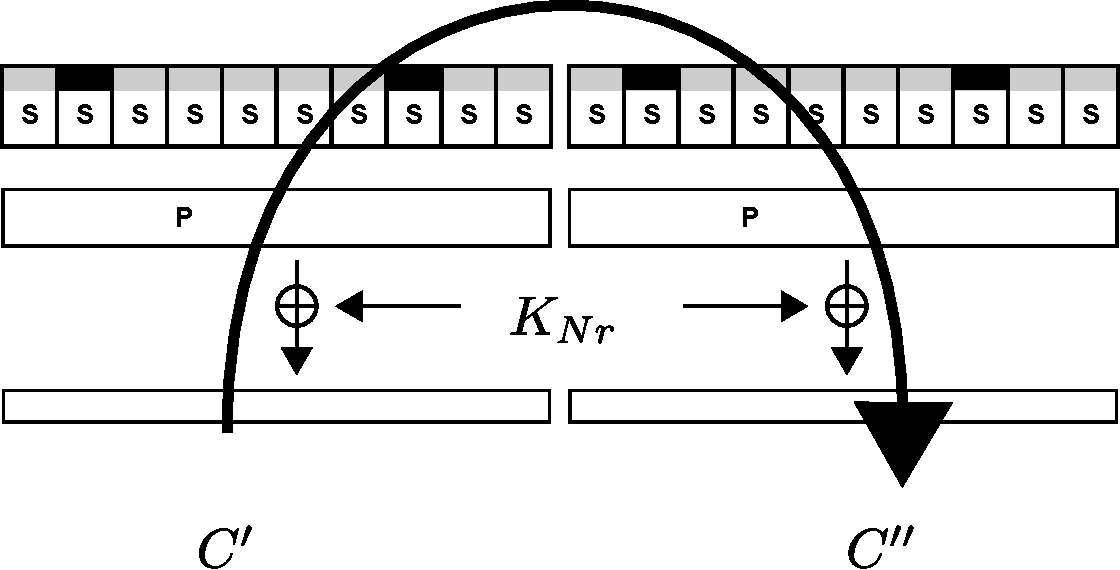
\includegraphics[width=.6\textwidth]{./attack-c.pdf}
 \caption{\emph{Attack-C} style equation system}
 \label{fig:attack-c}
\end{figure}


Again, we attempt to solve the system and wait for a fixed time $t$ to find a contradiction in the system. If no contradiction is found, we know that the pair $C',C''$ can be a right pair under some key. Thus we can consider \emph{Attack-C} as a quite expensive but thorough filter function: we invest more work in the management of the outer rounds using algebraic techniques.

Note that we cannot be certain about the output difference of the first round active S-Boxes or even that the differential $\delta_0 \rightarrow \delta_r$ holds. However, the attack can be adapted such that we can still recover key bits, for instance by considering multiple suggested right pairs. A second option is to attempt to solve the resulting smaller system to recover an encryption key candidate. Alternatively, we can execute the guess-and-verify step described above.

In order to gain more precise filters, we may add rounds prior to the round $r$ to our equation system. Instead of either stopping at round $r$ (counting from the rear) or going all the way as in \emph{Attack-B}, we may choose to add for example four more rounds prior to the round $r$. As Table~\ref{tab:present-bc} shows, this indeed improves the precision of the filter at the cost of being potentially more expensive.

\emph{Attack-C} has one caveat though. When we consider ciphers where the key-size is bigger than the block-size the solution space for the related ``cipher'' is significantly larger than for the original cipher. If we consider a 64-bit block-size cipher with a 128-bit key, two parallel executions of the cipher would be sufficient to uniquely determine the encryption key. However, the related ``cipher'' is effectively one execution of one 64-bit block-size cipher and thus not sufficient to actually determine the key.


\subsubsection{\emph{Symbolic Attack-C}.}
In \emph{Attack-C} the attacker considers an equation system only in those equations of the rounds $> r$. The attacker is thus left with $R$ rounds for each plaintext--ciphertext pair to consider; these are related by the output difference predicted by the differential. If we denote the equation system for the last $R$ rounds of the encryption of $P'$ to $C'$ and $P''$ to $C''$ as $F'_R$ and $F''_R$ respectively, then the algebraic part of \emph{Attack-C} is a Gröbner basis computation for the polynomial system $$F = F'_R \cup F''_R \cup \{X'_{r+1,i} \oplus X''_{r+1,i} \oplus \Delta X_{r+1,i} \mid 0 \leq i < B_s\}.$$ Note that we have no information except experimental evidence about how many pairs are actually discarded by this technique.

In order to get a lower bound, we consider the same system of equations as in \emph{Attack-C} but replace the tuples of constants $C'$ and $C''$ by tuples of symbols. If we then compute a Gröbner basis for the right elimination ordering (cf.\ Chapter~\ref{chapter:algebraic_features}), we can recover equations in the variables $C'$ and $C''$ which must evaluate to zero on the actual ciphertext values if the input difference for round $r+1$ holds. Once we recovered such equations we can calculate the probability that all these polynomials evaluate to zero for random values for $C'$ and $C''$ which gives an estimate about the quality of the filter.

\subsubsection{\emph{Attack-D}.}
The fraction of pairs which survive \emph{Attack-C} is determined by how many output differences $\Delta C = C' \oplus C''$ are impossible under the input difference $\delta_r$. As shown in Section~\ref{sec:present-symbolic-attack-c} the number of pairs rejected by \emph{Attack-C} drops rapidly if $R$, the number of ``free'' rounds, is increased. In \emph{Attack-C} we distinguish wrong pairs by discarding any pair which has an empty solution set for the related ``cipher''. Any pair which has at least \emph{one} solution is a candidate for a right pair. Consider the related ``cipher'' from \emph{Attack-C} as the function $\mathcal{E}: \F_2^b \times \F_2^k \to \F_2^b$, that is as a function taking a $k$-bit key and mapping a $b$-bit ``plaintext'' ($C'$) to the $b$-bit ``ciphertext'' ($C''$). We expect for a given a pair $C',C''$ on average $2^{k - b}$ keys which satisfy this pair; we expect $2^{k - b}$ keys to produce the same image $C''$ on average for a fixed $C'$. Now, assume \emph{Attack-C} accepts 1 in $2^a$ pairs for a given number of rounds $R$ and $\delta_r$. Then, for a given $C'$ we only have $2^{b - a}$ possible images $C''$ under $\mathcal{E}$ and we assume that on average $2^{k - (b - a)}$ keys will produce the same image $C''$ for a fixed $C'$.

For a given pair $C',C''$ we can estimate the size of the solution space using a technique inspired by the \texttt{MBound} model counter which is summarised in  \cite{Gomes-Sabharwal-Selman-2009} as follows:

\begin{quote}
The central idea of the approach is to use a special type of randomly chosen constrains (sic!), namely xor or parity constraints on the original variables of the problem. Such constraints require that an odd number of the involved variables be set to true. (This requirement can be translated into the usual CNF form by using additional variables, and can also be modified into requiring that an even number of variables be true by adding the constant 1 to the set of involved variables.) \texttt{MBound} works in a very simple fashion: repeatedly add a number $s$ of purely random xor constraints to the formula as additional CNF clauses, feed the resulting streamlined formula to a state-of-the-art complete SAT solver without any modification, and record whether or not the streamlined formula is still satisfiable. At a very high level, each random xor constraint will cut the solution space of satisfying assignments approximately in half. As a result, intuitively speaking, if after the addition of $s$ xor constraints the formula is still satisfiable, the original formula must have at least of the order of $2^s$ models. More rigorously, it can be shown that if we perform $t$ experiments of adding $s$ random xor constraints and our formula remains satisfiable in each case, then with probability at least $1 − 2^{−\alpha t}$ , our original formula will have at least $2^{s−\alpha}$ satisfying assignments for any $\alpha > 0$, thereby obtaining a lower bound on the model count with a probabilistic correctness guarantee. The confidence expression $1 − 2^{−\alpha t}$ says that by repeatedly doing more experiments (by increasing $t$) or by weakening the claimed bound of $2^{s−\alpha}$ (by increasing $\alpha$), one can arbitrarily boost the confidence in the lower bound count reported by this method.
\end{quote}


Thus, we can estimate the number of keys which satisfy a given map from $C'$ to $C''$. Experimental evidence suggests (cf.~Section~\ref{sec:adc}) that the expected values of $s$ for right pairs are bigger than for random pairs and are bounded away far from the expected values for $s$.

Based on this observation, we can either construct a more powerful filter to discard wrong pairs or rank candidate key counters (see Section~\ref{sec:attack-d-present}).

\section{The Block Cipher PRESENT}
\label{sec:present}
\textsc{Present} \cite{present} was proposed by A.~Bogdanov, L.R.~Knudsen, G.~Leander, C.~Paar, A.~Posch\-mann, M.J.B.~Robshaw, Y.~Seurin and C.~Vikkelsoe at CHES~2007 as an ultra-lightweight block cipher, enabling a very compact implementation in hardware, and therefore particularly suitable for RFIDs and similar devices. There are two variants of \PRESENT: one with 80-bit keys and one with a 128-bit keys, denoted as \PRESENT-80 and \PRESENT-128 respectively. In our experiments, we consider reduced round variants of both ciphers denoted as
\PRESENT-$K_s$-$N$, where $K_s \in \{80, 128\}$ represents the key size in bits and $1 \leq N \leq 31$ represents the number of rounds.

\PRESENT is an SP-network with a block-size of 64 bits and both versions have 31 rounds. Each round of the cipher has three layers of operations:  \texttt{keyAddLayer}, \texttt{sBoxLayer} and \texttt{pLayer}. The operation \texttt{keyAddLayer} is a simple subkey addition to the
current state, while the \texttt{sBoxLayer} operation consists of 16 parallel applications of a 4-bit S-Box given by $x \rightarrow S[x]$ where $ S = $[\texttt{C}, \texttt{5}, \texttt{6}, \texttt{B}, \texttt{9}, \texttt{0}, \texttt{A}, \texttt{D}, \texttt{3}, \texttt{E}, \texttt{F}, \texttt{8}, \texttt{4}, \texttt{7}, \texttt{1}, \texttt{2}]. The operation \texttt{pLayer} is a permutation of wires given by the rule that the bit at position $s \cdot j + i$ ($0 \leq j < B$, $0 \leq i < s$) is moved to position $B \cdot i + j$, where $s=4$ is the S-Box width and $B=16$ is the number of parallel S-Boxes.

In both versions, these three operations are repeated $N=31$ times. On the final round, an extra subkey addition is performed. The subkeys are derived from the user-provided key in the key schedule, which by design is also quite simple and efficient involving a cyclic right shift, one or two 4-bit S-Box applications (depending on the key size) and the addition of a round constant. For the 80-bit variant the user-supplied key is stored in a key register $K$ and represented as $k_{79} k_{78} \dots k_0$ . At round $i$ the 64-bit round key $K_i = k_{i,63} k_{i,62} \dots k_{i,0}$ consists of the 64 upmost bits of the current contents of register $K$: $K_i = k_{i,63} k_{i,62} \dots k_{i,0} = k_{79} k_{78} \dots k_{16}.$ After round key $K_i$ is extracted, the key register $k = k_{79} k_{78} \dots k_0$ is updated by a cyclic right shift, one S-Box application on the most significant four bits and a round counter addition to the bits 15 to 19. The key schedule for 128-bit keys is quite similar and presented in Appendix~II of \cite{present}. We note that the difference between the 80-bit and 128-bit variants is only the key schedule. In particular, both variants have the same number of rounds (i.e~$N=31$). The cipher designers explicitly describe in~\cite{present} the threat model considered when designing the cipher, and acknowledge that the security margin may be somewhat tight. Although they do not recommend immediate deployment of the cipher (especially the 128-bit version), they strongly encourage the analysis of both versions.

The \PRESENT authors give a security analysis of \PRESENT by showing resistance against well-known attacks such as differential and linear cryptanalysis \cite{present}. The best published ``classical'' differential attacks are for 16 rounds of \PRESENT-80 \cite{present-dc:africacrypt}. Results on linear cryptanalysis for up to 26 rounds are available in \cite{present-lc:eprint,present-lh}. Bit-pattern based integral attacks \cite{bit-pattern-ia} are successful up to seven rounds of \PRESENT. A new type of attack, called statistical saturation attack, was proposed in \cite{present-stat-sat} and shown to be applicable up to 24 rounds of \PRESENT.

\subsection{An Equation System for PRESENT}
\label{sec:present-equ}
One can compute 21 quadratic equations and one cubic equation for the S-Box of \PRESENT which form a \emph{degrevlex} Gr\"obner basis. This basis is used for all Gröbner basis computations in this chapter. Each round of \PRESENT introduces $2 \cdot 64$ new state variables for the input and output bits of the S-Box and thus we have $128 \cdot N$. The 80-bit key schedule has 80 user-provided key variables and 4 new key variables per round to account for one S-Box. Thus we have $N_v = (128 + 4) \cdot N + 80 = 132 \cdot N + 80$ variables. Each round gives rise to $22 \cdot 16$ S-Box equations, 64 key addition equations and 22 key schedule equations. We also have one additional key addition (64 linear equations) at the end and $N_v$ field equations of the form $x_i^2 + x_i = 0$.
Thus we have $$N_e = (22 \cdot 16 + 22 + 64) N + 64 + N_v = 570 \cdot N + 144$$ equations. If we use two plaintext--ciphertext pairs, we double the number of equations and variables for the state variables but not the number of equations and variables for the key variables\footnote{If the weight on the difference $\Delta P$ is small however, some variables for the first few rounds may be the same for both systems.}. Thus for \PRESENT-80-31 we would have a system of 8140 variables in 34742 equations if we consider two plaintext--ciphertext pairs. A generator for these equation systems is provided by the author at \url{http://bitbucket.org/malb/algebraic_attacks/src/tip/present.py}.

\subsection{Differential Cryptanalysis of 16 Rounds of PRESENT}
\label{sec:present-dc}

In the original proposal~\cite{present}, the designers of \PRESENT show that both linear and differential cryptanalysis are infeasible against the cipher. In \cite{present-dc:africacrypt,present-differentials} M.~Wang provides 24 explicit differential characteristics for 14 rounds. These hold with probability $2^{-62}$ and are within the theoretical bounds provided by the \PRESENT designers. Wang's attack is reported to require $2^{64}$ memory accesses to cryptanalyse 16 rounds of \PRESENT-80. We use his characteristics to mount our attack. Furthermore, we also make use of and compare to the filter function presented in \cite{present-dc:africacrypt}, which we briefly describe below.

Consider for example the differential characteristic provided in \cite{present-dc:africacrypt}. It ends with the difference $\delta = \texttt{1001} = \texttt{9}$ as input for the two active S-Boxes of round 15. According to the difference distribution table of the \PRESENT S-Box, the possible output differences are \texttt{2}, \texttt{4}, \texttt{6}, \texttt{8}, \texttt{C} and \texttt{E}. This means that the least significant bit is always zero and the weight of the output difference (with the two active S-Boxes) is at most 6. It then follows from \texttt{pLayer} that at most six S-Boxes are active in round 16. Thus we can discard any pair for which the outputs of round 16 have non-zero difference in the positions arising from the output of S-Boxes other than the active ones. There are ten inactive 4-bit S-Boxes, and we expect a pair to pass this test with probability $2^{-40}$.

Furthermore, it also follows from \texttt{pLayer} that the active S-Boxes in round 16 (of which there are at most six, as described above) will have input difference $\texttt{1}$ and thus all possible output differences are $\texttt{3}$, $\texttt{7}$, $\texttt{9}$, $\texttt{D}$ (and $\texttt{0}$, in case the S-Box is inactive). Thus we can discard any pair not satisfying these output differences for these S-Boxes. We expect a pair to pass this test with probability $\frac{16}{5}^{-6} = 2^{-10.07}$. Overall we expect pairs to pass both tests with probability $2^{-50.07}$. We expect to be able to construct a similar filter function for all the 24 differential characteristics presented in \cite{present-differentials}.

\section{The Block Cipher KTANTAN32}
\label{sec:ktantan32}
KTANTAN32 \cite{CDK09} is the smallest cipher in a family of block ciphers proposed at CHES~2009 by Christophe de Canniere, Orr Dunkelman, and Miroslav Knezevic. It has a block-size of 32 bits and accepts an 80-bit key. The input is loaded into two registers $L_2$ and $L_1$ of 19 and 13 bit length respectively and then a round transformation is applied to these registers 254 times. This round function is
\begin{algorithm}
$r_a \longleftarrow L_1[12] \oplus L_1[7] \oplus (L_1[8] \cdot L_1[5]) \oplus L_1[3] \cdot t \oplus k_a$\;
$r_b \longleftarrow L_2[18] \oplus L_2[7] \oplus (L_2[12] \cdot L_2[10]) \oplus (L_2[8] \cdot L_2[3]) \oplus k_b$\;
$L_1 \longleftarrow L_1 \ggg 1$; $L_1[0] \longleftarrow r_b$\;
$L_2 \longleftarrow L_2 \ggg 1$; $L_2[0] \longleftarrow r_a$\;
\end{algorithm}

In the above description $L_1$ and $L_2$ are represented in little-endian bit ordering, $k_a$ and $k_b$ are key bits selected by a non-linear function and $t$ is a round constant. After 254 rounds the content of $L_2$ and $L_1$ is output as the ciphertext. The description of KTANTAN32 gives rise to a straight-forward algebraic description of the cipher which introduces two new variables per round for $r_a$ and $r_b$. In our experiments we consider round-reduced variants of KTANTAN32 which we denote KTANTAN32-$N$ where $N$ is the number of rounds.

The designers of KTANTAN consider a wide range of attacks in their security argument and showed the cipher secure against differential, linear, impossible differential, algebraic attacks and some combined attacks. In particular, the designers show that there is no differential characteristic for 42 rounds with probability better than $2^{-11}$. 

\subsection{A Differential Characteristic for KTANTAN32}
\label{sec:ktantan32-characteristic}
The designers provided us with the best explicit characteristic for the first 42 rounds in private communication. Using a simple heuristic -- always choosing a zero output difference if there is a choice -- this characteristic can be extended to 71 rounds with probability $2^{-31}$ disregarding any dependencies. This characteristic is given in Figure~\ref{fig:ktantan32-characteristic}.

\begin{figure}[ht]
\begin{center}
\begin{minipage}{0.6\textwidth}
\begin{verbatim}
                L2               L1
INP   0 0000000100010101011 0000000001000
  1   0 0000000010001010101 0000000000100                                   
  2   1 0000000001000101010 0000000000010                                 
  3   1 0000000000100010101 0000000000001
  4   2 1000000000010001010 0000000000000
  5   2 0100000000001000101 0000000000000
...                                      
 42  12 0000001000010000000 0001000000000
 43  12 0000000100001000000 0000100000000
 44  13 0000000010000100000 0000010000000
 45  15 0000000001000010000 0000001000000
...                                      
 71  31 0000000010000100010 0000000000000
\end{verbatim}
\end{minipage}
\end{center}
\caption{71 round characteristic for KTANTAN32}
\label{fig:ktantan32-characteristic}
\end{figure}


\section{Experimental Results}
\label{sec:adc}
In this section we give experimental evidence for the viability of the attacks developed so far in this chapter. All attacks in this section were implemented in the mathematics software Sage \cite{sage}. We will start with the \emph{Symbolic Attack-C} and the \emph{Generalised Attack-B} since we will use them in later attacks.

We note that it is non-trivial to estimate the time complexity of the attacks discussed in this chapter. Except for successfully mounting an attack against the target cipher it is rather difficult to estimate how long on average Gröbner basis algorithms and SAT solvers will take to solve a given family of systems. In order to estimate the running time of our attacks, we will test them against three classes of pairs:
\begin{enumerate}
 \item Random pairs will constitute the overwhelming majority. Thus, the time it takes to reject a random candidate pair is a significant indicator of the performance of the attack. However, we know that a certain fraction of random pairs can be filtered using \emph{Symbolic Attack-C} whose cost can be estimated quite accurately. Thus we also consider random pairs which survive this filter.
 \item Right pairs for the differential but not necessarily the characteristic are expected to be difficult candidates. Thus, they should provide an upper limit on the runtime. For differentials with reasonably high probability, we generated these pairs using a brute-force search via our bit-sliced implementation\footnote{provided by at \url{http://bitbucket.org/malb/algebraic_attacks/src/tip/present_bitslice.c}} of \PRESENT. That is, we tried about $2^{45}$ pairs and tested whether they have the output difference after 10 rounds we are looking for.
 \item Right pairs for the characteristic can be constructed efficiently using a SAT solver up to a number of rounds as shown in \cite{alg-des}. We give a selection of right pairs for the characteristic from \cite{present-dc:africacrypt} constructed this way in Table~\ref{tab:present80-right-pairs}. It might be considered problematic to generate challenge data using the same technique which is used to solve these pairs since there might be some hidden algebraic structure due to this generation process. However, we assume that no hidden algebraic structure is produced. This is because we pick a random key first and then search for plaintext and ciphertext values such that the characteristic is satisfied. If the probability of the characteristic is close to $2^{-b}$ where $b$ is the blocksize of the cipher, we expect very few degrees of freedom for the SAT solver. In Table~\ref{tab:present80-right-pairs} we consider a characteristic which holds with probability $2^{-62}$ for a 64-bit blocksize. Thus, we expect only 4 right pairs on average after we fixed a key.
\end{enumerate}


\begin{table}
\begin{center}
\begin{tabular}{|c|c|}
\hline
$P'$ & $K$\\
\hline
\texttt{c61bf05c 2a39a5e4} & \texttt{11ec9f16 5edf2206 2eca}\\
\texttt{0538a885 efcc1610} & \texttt{7d227785 08f40902 5443}\\
\texttt{7ff2f485 d5a60d21} & \texttt{e0d9bb12 8807920c 5c08}\\
\texttt{cf9237a3 59636e00} & \texttt{076561d0 4cbd0675 3ee3}\\
\texttt{e9cb5753 e695ef32} & \texttt{4e7cacde 64f8a099 7656}\\
\texttt{adfaf8c6 df732dcf} & \texttt{b53f5586 0b516585 67e8}\\
\texttt{66396df4 366faa43} & \texttt{69b319cb 18b56d0d 2d97}\\
\texttt{25fd6008 9c1bdbfc} & \texttt{05f0e912 e477c457 2bb5}\\
\texttt{544841b2 ce90aa14} & \texttt{1bd3681c eee2ea8d d2e0}\\
\texttt{530c3275 4d0d666f} & \texttt{d403c614 1c074ef5 a629}\\
\texttt{a283ce93 eab76c9d} & \texttt{0d6b63e5 dd806b00 6ef8}\\
\texttt{a1637f3f 6a497c75} & \texttt{b6005536 8fccfbcc ff6f}\\
\texttt{76c6fc0d b9e541ac} & \texttt{2e1f1d8b 46ee7986 3c59}\\
\texttt{7d6f4036 11cfe536} & \texttt{9544bc1c 16dfaddc a8ca}\\
\texttt{0e1fc0e1 43c74365} & \texttt{f952e6db c3c89b47 64a4}\\
\texttt{1eea7d43 37962d04} & \texttt{0eb932ae ae36e58d 1f57}\\
\texttt{26e3ed68 a0f4a62d} & \texttt{218027b0 d3579e80 0321}\\
\texttt{8f5c5ca1 ee230995} & \texttt{c808951c c403fefc 016e}\\
\texttt{a9e16caa 327d0361} & \texttt{f6cd9ff8 7224946e a4db}\\
\texttt{2c795566 739e1b06} & \texttt{bc05d993 8ea6e4f7 f8fb}\\
\texttt{a283ce93 eab76c9d} & \texttt{0d6b63e5 dd806b00 6ef8}\\
\texttt{76c6fc0d b9e541ac} & \texttt{2e1f1d8b 46ee7986 3c59}\\
\texttt{26e3ed68 a0f4a62d} & \texttt{218027b0 d3579e80 0321}\\
\texttt{8f5c5ca1 ee230995} & \texttt{c808951c c403fefc 016e}\\
\texttt{a9e16caa 327d0361} & \texttt{f6cd9ff8 7224946e a4db}\\
\texttt{2c795566 739e1b06} & \texttt{bc05d993 8ea6e4f7 f8fb}\\
\texttt{b9d5ee1a 9ec8298b} & \texttt{c6d9fb3e 9cc686df 69ab}\\
\texttt{e09f9557 3a01e584} & \texttt{877b6b0b 203fe2f0 fde3}\\
\hline
\end{tabular}
\end{center}
\caption{Right pairs for the 14 round characteristic \cite{present-dc:africacrypt} for \PRESENT-80.}
\label{tab:present80-right-pairs}
\end{table}


\subsection{\emph{Symbolic Attack-C} and the Quality of \emph{Attack-C} against PRESENT}
\label{sec:present-symbolic-attack-c}
We consider the differential from \cite{present-dc:africacrypt} and construct filters for \PRESENT reduced to $14 + R$ rounds; the same filter applies also to $10 + R$ and $6 + R$ rounds since the characteristic is iterative with a period of four rounds. The explicit polynomials in this section do not differ for \PRESENT-80 and \PRESENT-128.

\subsubsection*{1R}
We construct the polynomial ring $P = $
\begin{displaymath}
\begin{array}{lll}\F_2[&K_{0,0},\dots, K_{0,79}, &
K_{1,0},\dots,K_{1,3},\\
&Y'_{1,0}, \dots,Y'_{1,63},  & Y''_{1,0}, \dots,Y''_{1,63}, \\
&X'_{1,0}, \dots,X'_{1,63}, & X''_{1,0}, \dots,X''_{1,63},\\
&\dots,& K_{15,0},\dots,K_{15,3},\\
& Y'_{15,0}, \dots,Y'_{15,63}, & Y''_{15,0}, \dots,Y''_{15,63},\\
& X'_{15,0}, \dots,X''_{15,63}, & X''_{15,0}, \dots,X''_{15,63},\\
& C'_{0}, \dots,C'_{63}, & C''_{0}, \dots,C''_{63}]\end{array}
\end{displaymath}
and attach the following block ordering:
\begin{displaymath}
\underbrace{K_{0,0}, \dots,X''_{15,63}}_\textnormal{degrevlex},
\underbrace{C'_{0}, \dots,C''_{63}, C''_{0},
\dots,C''_{63}}_\textnormal{degrevlex}.
\end{displaymath}

We set up an equation system as in \emph{Attack-C} except that the ciphertext bits are symbols ($C'_{i}$ and $C''_{i}$). Then, we compute the Gröbner basis up to degree $D=3$ using \PolyBoRi 0.6.3 \cite{polybori} with the option \texttt{deg\_bound=3} and filter out any polynomial that contains non-ciphertext variables.

This computation returns 60 polynomials of which 58 are linear. These 58 linear polynomials are of the form $C'_{i} + C''_{i}$ for 
$$
i \in \{0,\dots,6, 8, \dots 14, 16, \dots 22, 24, \dots 30, 32, \dots 38, 40, \dots 46, 48, \dots, 63\}.
$$
The remaining two polynomials are $$(C'_{23} + C''_{23} + 1)(C'_{7} + C'_{39} + C''_{7} + C''_{39} + 1)$$ and 
$$(C'_{31} + C''_{31} + 1)(C'_{15} + C'_{47} + C''_{15} + C''_{47} + 1).$$

The probability that all polynomials evaluate to zero on a random point is $2^{-58.83}$. A random point is a point where we choose the bits of $C'$ and $C''$ at random.

\subsubsection*{2R Attack}

We extend the ring from the 1R experiment in the obvious way, set up an \emph{Attack-C} style equation system in the
same fashion and compute a Gröbner basis where we ignore any S-polynomial with degree greater than $3$ as before.

This computation returns 65 polynomials of which 46 are linear. Forty linear polynomials are of the form $C'_{i} + C''_{i}$ and encode the information that the last round output difference of 10 S-Boxes must be zero (cf. \cite{present-dc:africacrypt}). The remaining 24 polynomials split into two groups $F_0,F_2$ of 12 (ignoring a 13th polynomial for the moment) polynomials in 24 variables each and the $F_j$ do not share any variables with each other or the first 40 linear polynomials.
\begin{align*}
& (C'_{57+j} + C''_{57+j})    (C'_{53+j} + C''_{53+j} + 1)(C'_{17+j} + C''_{17+j}),\\
& (C'_{57+j} + C''_{57+j})    (C'_{53+j} + C''_{53+j} + 1)(C'_{33+j} + C''_{33+j}),\\
& (C'_{57+j} + C''_{57+j} + 1)(C'_{25+j} + C''_{25+j}),\\
& (C'_{57+j} + C''_{57+j} + 1)(C'_{41+j} + C''_{41+j}),\\
& (C'_{53+j} + C''_{53+j} + 1)(C'_{21+j} + C''_{21+j}),\\
& (C'_{53+j} + C''_{53+j} + 1)(C'_{37+j} + C''_{37+j}),\\
& (C'_{53+j} + C''_{53+j} + 1)(C'_{49+j} + C'_{57+j} + C''_{49+j} + C''_{57+j} + 1),\\
& (C'_{49+j} + C''_{49+j} + 1)(C'_{17+j} + C''_{17+j}),\\
& (C'_{49+j} + C''_{49+j} + 1)(C'_{33+j} + C''_{33+j}),\\
& C'_{ 1+j} + C'_{33+j} + C'_{49+j} + C''_{ 1+j} + C''_{33+j} + C''_{49+j},\\
& C'_{ 5+j} + C'_{37+j} + C'_{53+j} + C''_{ 5+j} + C''_{37+j} + C''_{53+j},\\
& C'_{ 9+j} + C'_{41+j} + C'_{57+j} + C''_{ 9+j} + C''_{41+j} + C''_{57+j}.\\
\end{align*}

Furthermore, the computation returned $$(C'_{51} + C''_{51} + 1)(C'_{35} + C''_{35} + 1)(C'_{19} + C''_{19}).$$
This asymmetry is an artefact of the effectively random abort induced by the $D=3$ bound. We add a polynomial of this form to both sets and
get that the probability that all 66 polynomials evaluate to zero for a random point is $\approx 2^{-50.669}$. 

If we construct random pairs $C',C''$ which pass this filter, \emph{Attack-C} will reject roughly every second pair for \PRESENT-80 and $195$ out of $512$ for \PRESENT-128. Thus we expect \emph{Attack-C} to pass with probability $\approx 2^{-51.669}$  for \PRESENT-80 and with probability $\approx 2^{-51.361}$ for \PRESENT-128.

For comparison recall that Wang's filter from \cite{present-dc:africacrypt} passes with probability $2^{-40} \cdot (5/16)^6 \approx 2^{-50.07}$.

\subsubsection*{3R Attack}
We extend the ring and the block ordering in the obvious way and compute a Gröbner basis with degree bound 3. The computation returns 28 polynomials of which 16 are linear. The linear polynomials have the form $C'_{i} + C''_{i}$ for $$i \in
\{3,7,11,15,19,23,27,31,35,39,43,47,51,55,59,63\}.$$

The remaining $12$ polynomials are:
\begin{eqnarray*}
&(C'_{36} + C''_{36})((C'_{ 4} + C''_{4})(C'_{20} + C'_{52} + C''_{20} + C''_{52} + 1) +  (C'_{20}+C''_{20}+1)(C'_{52} + C''_{52}+1)),\\
&(C'_{37} + C''_{37})((C'_{ 5} + C''_{ 5})(C'_{21} + C'_{53} + C''_{21} + C''_{53} + 1) + (C'_{21} + C''_{21} + 1)(C'_{53} + C''_{53} + 1)),\\
&(C'_{40} + C''_{40})((C'_{ 8} + C''_{ 8})(C'_{24} + C'_{56} + C''_{24} + C''_{56} +1) + (C'_{24} + C''_{24} + 1)(C'_{56} + C''_{56} + 1)),\\
&(C'_{41} + C''_{41})((C'_{ 9} + C''_{ 9})(C'_{25} + C'_{57} + C''_{25} + C''_{57} +1) + (C'_{25} + C''_{25} + 1)(C'_{57} + C''_{57} + 1)),\\
&(C'_{45} + C''_{45})((C'_{13} + C''_{13})(C'_{29} + C'_{61} + C''_{29} + C''_{61} + 1) + (C'_{29} + C''_{29} + 1)(C'_{61} + C''_{61} + 1)),\\
&(C'_{46} + C''_{46})((C'_{14} + C''_{14})(C'_{30} + C'_{62} + C''_{30} + C''_{62} + 1) + (C'_{30} + C''_{30} + 1)(C'_{62} + C''_{62} + 1)),\\
& (C'_{06} + C''_{06})((C'_{22} + C''_{22})(C'_{38} + C'_{54} + C''_{38} + C''_{54} + 1) + (C'_{38} + C''_{38} + 1)(C'_{54} + C''_{54} + 1)),\\
& (C'_{10} + C''_{10})((C'_{26} + C''_{26})(C'_{42} + C'_{58} + C''_{42} + C''_{58} + 1) + (C'_{42} + C''_{42} + 1)(C'_{58} + C''_{58} + 1)),\\
& (C'_{12} + C''_{12})((C'_{28} + C''_{28})(C'_{44} + C'_{60} + C''_{44} + C''_{60} + 1) + (C'_{44} + C''_{44} + 1)(C'_{60} + C''_{60} + 1)),\\
& (C'_{52} + C''_{52} + 1)(C'_{20} + C''_{20} + 1)(C'_{ 4} + C'_{36} + C''_{ 4} + C''_{36}),\\
& (C'_{60} + C''_{60} + 1)(C'_{28} + C''_{28} + 1)(C'_{12} + C'_{44} + C''_{12} + C''_{44}),\\
& (C'_{10} + C'_{42} + C'_{58} + C''_{10} + C''_{42} + C''_{58})(C'_{ 2} + C'_{34} + C'_{50} + C''_{ 2} + C''_{34} + C''_{50}).\\
\end{eqnarray*}

The probability that all polynomials evaluate to zero on a random point is $\approx 2^{-18.296}$.

If we construct random pairs $C',C''$ which pass this filter, \emph{Attack-C} will accept roughly $6$ in $1024$ for \PRESENT-80 and $9$ out of $1024$ for \PRESENT-128. Thus we expect \emph{Attack-C} to pass with probability $\approx 2^{-25.711}$ for \PRESENT-80 and $2^{-25.126}$ for \PRESENT-128.

\subsubsection*{4R Attack}
We extend the ring and the block ordering in the obvious way. With a degree bound $D=3$ we recover $$(C'_{32+j} + C''_{32+j} + 1)(C'_{j} + C''_{j} + 1)(C'_{16+j} + C'_{48+j} + C''_{16+j} + C''_{48+j})$$ for $0 \leq j < 16$. The probability that all polynomials evaluate to zero on a random point is $\approx 2^{-3.082}$. We verified experimentally that this bound is almost optimal by using the SAT solver \CryptoMiniSat on \emph{Attack-C} systems and a 4R attack against \PRESENT-80-14. Using this solver we verified that a random such system has a solution with probability $\approx 2^{-3}$. Thus, we conclude that \emph{Attack-C} will roughly accept 1 in 8 pairs.

\subsection{\emph{Symbolic Attack-C} against KTANTAN32}
In Tables~\ref{tab:ktantan32-c-4} and \ref{tab:ktantan32-c-5} we give our results against KTANTAN32. These results use the characteristic from Section~\ref{sec:ktantan32-characteristic}. We present results for the degree bounded at four and at five respectively. For each degree bound we give the number of degree $d=1-5$ polynomials. In the last column of each experiment we give the logarithm of the approximate probability that all the equations we found evaluate to zero for random values (denoted $\log_2 p$).

\begin{table}
\begin{small}
 \begin{center}
\begin{tabular}{|l|r|r|r|r|r|r|}
\hline
$N$ & $d=1$ & $d=2$ & $d=3$ & $d=4$ & $d=5$& $\log_2 p$\\
\hline
 72 & 32 &  0 &   0 &   0 & 0 & ${-32.0}$\\                                                                                                                                         
 74 & 32 &  0 &   0 &   0 & 0 & ${-32.0}$\\                                                                                                                                         
 76 & 32 &  0 &   0 &   0 & 0 & ${-32.0}$\\                                                                                                                                         
 78 & 31 &  3 &   0 &   0 & 0 & ${-32.0}$\\
 80 & 28 & 11 &   0 &   0 & 0 & ${-31.4}$\\
 82 & 25 & 23 &   0 &   0 & 0 & ${-31.0}$\\
 84 & 20 & 32 &   4 &   8 & 0 & ${-29.0}$\\
 86 & 16 & 44 &  19 &   8 & 0 & ${-25.7}$\\
 88 & 12 & 39 &  54 &  96 & 0 & ${-24.0}$\\
 90 &  8 & 41 & 129 & 287 & 0 & ${-23.0}$\\
 92 &  4 & 28 & 113 & 285 & 0 & ${-20.0}$\\
 94 &  1 & 20 &  94 & 244 & 0 & ${-16.3}$\\
 96 &  0 &  8 &  38 &  96 & 0 & ${-12.8}$\\
 98 &  0 &  3 &   8 &  29 & 0 & ${-7.0 }$\\
 99 &  0 &  2 &   5 &  22 & 0 & ${-5.1 }$\\
100 &  0 &  1 &   3 &  13 & 0 & ${-3.7 }$\\
101 &  0 &  1 &   2 &   6 & 0 & ${-1.8 }$\\
102 &  0 &  0 &   0 &   2 & 0 & ${-0.8 }$\\
103 &  0 &  0 &   0 &   1 & 0 & ${-0.4 }$\\
104 &  0 &  0 &   0 &   0 & 0 &   ${0.0}$\\
\hline                                          
\end{tabular}                             
\end{center}
\end{small}
\caption{\emph{Symbolic Attack-C} against KTANTAN32 with degree bound 4.}
\label{tab:ktantan32-c-4}
\end{table}



\begin{table}
\begin{small}
 \begin{center}
\begin{tabular}{|l|r|r|r|r|r|r|}
\hline
$N$ & $d=1$ & $d=2$ & $d=3$ & $d=4$ & $d=5$& $\log_2 p$\\
\hline
 72 &  32 &  0 &   0 &   0 &    0&   ${-32.0}$\\                                                                                                                                         
 74 &  32 &  0 &   0 &   0 &    0&   ${-32.0}$\\                                                                                                                                         
 76 &  32 &  0 &   0 &   0 &    0&   ${-32.0}$\\                                                                                                                                         
 78 &  31 &  3 &   0 &   0 &    0&   ${-32.0}$\\
 80 &  28 & 11 &   0 &   0 &    0&   ${-31.4}$\\
 82 &  25 & 23 &   0 &   0 &    0&   ${-31.0}$\\
 84 &  20 & 32 &   4 &  32 &    0&   ${-29.0}$\\
 86 &  16 & 46 &  23 &  75 &  106&    $\leq -25.7$\\
 88 &  12 & 51 & 103 & 371 &  745&    $\leq -24.0$\\
 90 &   8 & 42 & 133 & 612 & 1762&    $\leq -23.0$\\
 92 &   4 & 33 & 133 & 743 & 2646&   ${-20.4}$\\
 94 &   1 & 25 & 124 & 662 & 2345&   ${-18.5}$\\
 96 &   0 &  8 &  52 & 287 & 1264&   ${-14.3}$\\
 98 &   0 &  3 &  10 &  46 &  156&   ${- 9.1}$\\
 99 &   0 &  2 &   5 &  32 &   85&   ${- 6.6}$\\
100 &   0 &  1 &   3 &  18 &   47&   ${- 4.6}$\\
101 &   0 &  1 &   2 &   8 &   19&   ${- 1.9}$\\
102 &   0 &  0 &   0 &   4 &    9&   ${- 0.9}$\\
103 &   0 &  0 &   0 &   2 &    4&   ${- 0.4}$\\
104 &  N/A& N/A&  N/A&  N/A&  N/A&         N/A\\
\hline                                          
\end{tabular}                             
\end{center}
\end{small}
\caption{\emph{Symbolic Attack-C} against KTANTAN32 with degree bound 5.}
\label{tab:ktantan32-c-5}
\end{table}

\subsection{\emph{Attack-D} against PRESENT}
\label{sec:attack-d-present}
We consider a 4R attack against \PRESENT-80-18 and against \PRESENT-80-14 as well as a 3R attack against \PRESENT-80-13. Considering the 4R attack on \PRESENT-80-18, we know that \emph{Attack-C} will accept roughly 1 in 8 pairs. Thus, we expect on average $2^{80 - (64 - 3)} = 2^{19}$ keys to satisfy a given map $C' \rightarrow C''$ for the related ``cipher'' constructed in \emph{Attack-C}. We denote the equation system implied by the map $C' \rightarrow C''$ as $F$ in this subsection.

We ran experiments for 1920 different pairs where we kept adding linear polynomials with $k=4$ randomly chosen variables to $F$ until the system was not soluble any more and recorded the maximum number $s$ of linear equations where the system was still soluble. Four variables were chosen because of performance reasons. We ran $t=10$ such experiments for each pair and then took the average value to reduce the impact of measurement imprecisions since $k=4$ is rather low.

For the 4R attack on \PRESENT-80-14, we expect roughly 1 in 8 pairs to survive, thus we expect $2^{80 - (64-3)} = 2^{19}$ keys per surviving pair just as before. We ran 597 experiments with $k=4$ and $t=10$.

For the 3R attack on \PRESENT-80-13, we expect roughly 1 in $2^{25}$ pairs to survive, thus we expect $2^{80 - (64-25)} = 2^{41}$ keys per surviving pair. We ran 1066 experiments with $k=3$ and $t=5$.

A crucial question is how to approximate the observed distribution. A case can be made for the Poisson distribution, at least if we consider $t=1$.
\begin{itemize}
 \item We have a discrete distribution of small integers.
 \item The value $s$ is the number of successful "yes/no" experiments where we test whether adding a number of linear polynomials makes the system unsolvable.
 \item In the 4R experiments the variance is relatively close to the mean. The Poisson distribution has a variance equal to the mean.
\end{itemize}

However, there are convincing arguments against the Poisson distribution as well:
\begin{itemize}
 \item Contrary to a Poisson distribution, our experiments are not independent, since the probability that $i+1$ linear equations will be solvable when $i$ polynomials are not solvable is low (but not zero due to the low value for $k$).
 \item In the 3R attack the integers are not that small anymore. 
 \item In the 3R attack the variance is far from the mean.
 \item If we consider the average of $t>1$ experiments per pair, we get a finer resolution than for a Poisson distribution.
\end{itemize}

Thus, an argument can be made for the normal distribution. In the following, we approximate the distribution by the normal distribution. We stress however  that this approximation might be too optimistic.

In Figure~\ref{fig:present-80-18-14-attack-d-histogram} and \ref{fig:present-80-13-10-attack-d-histogram} we plot the histogram for the values of $s$ for random pairs passing the filter from \emph{Attack-C} against the expected curves of the normal distribution. For the 4R attack on \PRESENT-80-18 we have $\mu=15.300$, $\sigma=3.065$ and $\sigma^2=9.393$. For the 4R attack on \PRESENT-80-14 we get $\mu=15.450$, $\sigma=3.244$ and $\sigma^2=10.521$. For the 3R attack we have $\mu=39.838$, $\sigma=2.997$ and $\sigma^2=8.980$. We note that both for the 3R and the 4R case $\mu$ ($15.45$ and $39.84$) is smaller than the value we would expect from the general argument made earlier ($19$ and $41$).

Under the assumption that the normal distribution is a reasonable approximation, we can estimate the probability that a random pair is still satisfiable if we add a given number of linear polynomials. These probabilities are given in Table~\ref{tab:present-80-18-14-attack-d-prob} and \ref{tab:present-80-13-10-attack-d-prob}.

\begin{figure}[htbp]
 \centering
 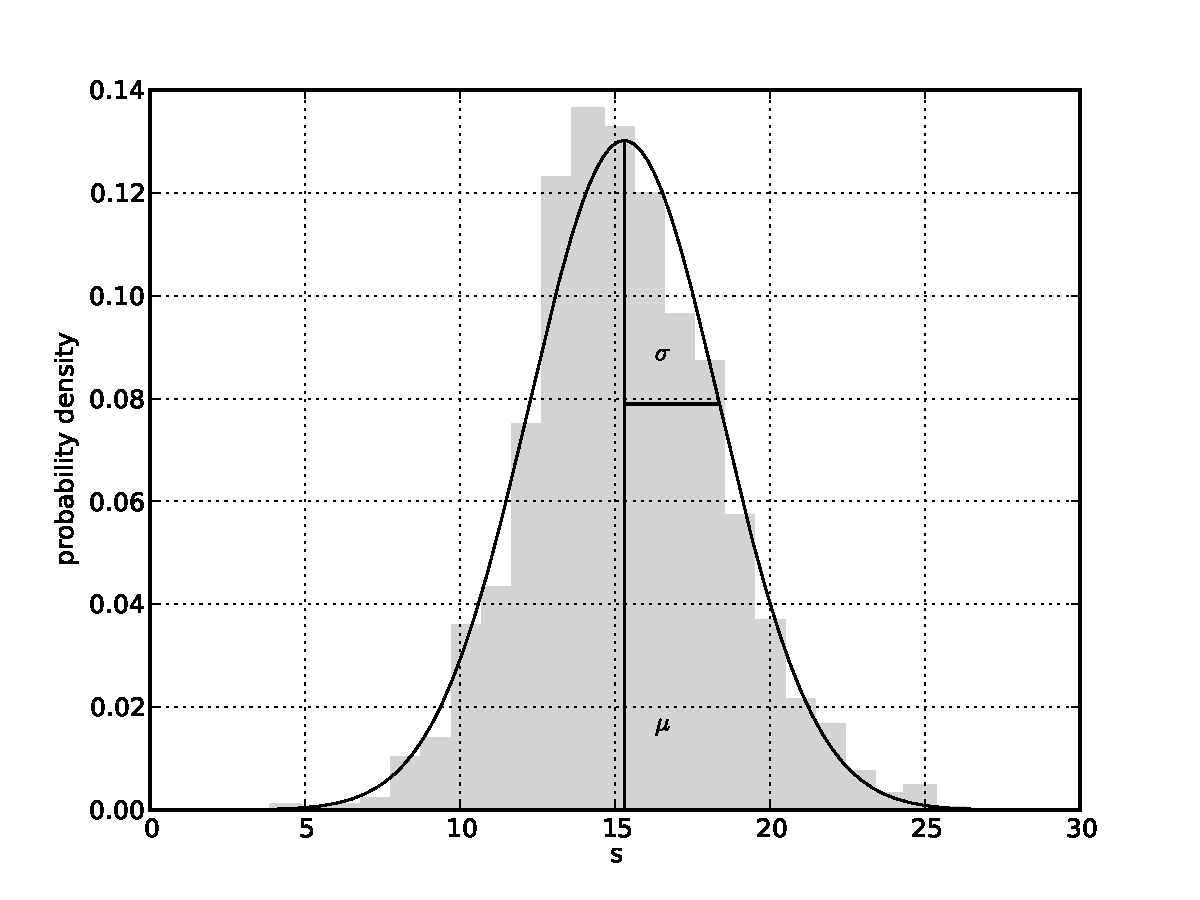
\includegraphics[width=0.9\textwidth]{./present-80-18-14-attack-d-histogram.pdf}
 \caption{4R \emph{Attack-D} on \PRESENT-80-18}
 \label{fig:present-80-18-14-attack-d-histogram}
\end{figure}

\begin{figure}[htbp]
 \centering
 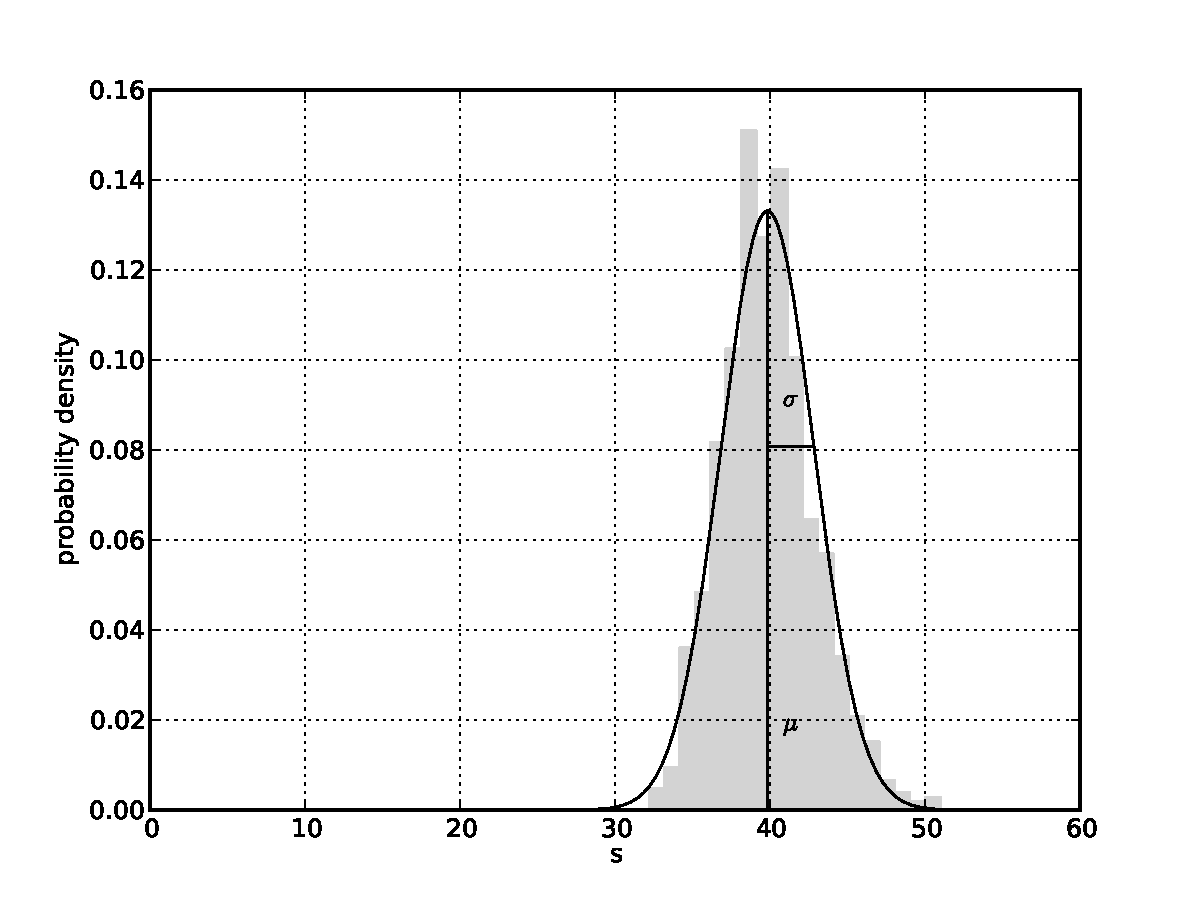
\includegraphics[width=0.9\textwidth]{./present-80-13-10-attack-d-histogram.pdf}
 \caption{3R \emph{Attack-D} on \PRESENT-80-13}
 \label{fig:present-80-13-10-attack-d-histogram}
\end{figure}

\begin{table}[ht]
\begin{center}
\begin{tabular}{|r|r|r|r|r|r|r|r|r|r|r|}
\hline
$s$                         & 22 & 23 & 24 & 25 & 26 & 27 & 28 & 29 & 30 & 31\\  
\hline
$\log_2 \textnormal{Pr}(s)$ & -4.11 & -4.97 & -5.92&  -6.98 & -8.13& -9.39 & -10.76 & -12.23 & -13.80 & -15.48\\
\hline
\end{tabular}
\end{center}
\caption{Probabilities for 4R \emph{Attack-D} against \PRESENT-80-18.}
\label{tab:present-80-18-14-attack-d-prob}
\end{table}


\begin{table}[ht]
\begin{center}
\begin{tabular}{|r|r|r|r|r|r|r|r|r|r|r|}
\hline
$s$                         &   44 &    45 &    46 &    47 &    48 &    49 &    50 &     51 &     52 &     53\\
\hline
$\log_2 \textnormal{Pr}(s)$ & -2.78 & -3.60 & -4.56 & -5.65 & -6.89 & -8.27 & -9.81 & -11.49 & -13.32 & -15.31\\
\hline
\end{tabular}
\end{center}
\caption{Probabilities for 3R \emph{Attack-D} against \PRESENT-80-13.}
\label{tab:present-80-13-10-attack-d-prob}
\end{table}

To check the accuracy of the prediction in Table~\ref{tab:present-80-18-14-attack-d-prob} we tested 1024 random pairs for \PRESENT-80-18 whether they are still solvable with $s=26$. Four of 1024 pairs survived; while the Gauss formulae predicted $2^{10} \cdot 2^{-8.13} \approx 4$ pairs.

By inspection of the Tables~\ref{tab:present-80-14-attack-d} and \ref{tab:present-80-18-attack-d} we can see that right pairs follow a different distribution. Right pairs for \PRESENT-80-18 have $\mu = 28.60$ and $\sigma = 6.55$ (for $t=10$ and $k=4$). Right pairs for \PRESENT-80-14 have  $\mu = 27.71$ and $\sigma=5.09$ (for $t=10$ and $k=3$).

\begin{table}[ht]
\begin{center}
\begin{tabular}{|c|c||r|r|r||r|r|r||r|r|r|}
\hline
Key & Char & \multicolumn{3}{|c||}{2R} & \multicolumn{3}{|c||}{3R} &  \multicolumn{3}{|c|}{4R}\\
\hline
& & $\lfloor s \rfloor$ & $\lfloor s \rceil$ & $\lceil s \rceil$ & $\lfloor s \rfloor$ & $\lfloor s \rceil$ & $\lceil s \rceil$ & $\lfloor s \rfloor$ & $\lfloor s \rceil$ & $\lceil s \rceil$ \\
\hline
\texttt{fc676e7c dad721db 95c7} & 0 & 67 & 69 & 73 & 48 & 50 & 52 & 28 & 30 & 34\\
\hline
\texttt{8e96e4d8 233c16b6 95bc} & 0 & 71 & 73 & 76 & 59 & 60 & 61 & 34 & 37 & 41\\
                                & 1 & 69 & 69 & 71 & 49 & 50 & 52 & 22 & 23 & 26\\
                                & 0 & 72 & 75 & 80 & 65 & 67 & 69 & 44 & 44 & 44\\
\hline
\texttt{04175372 9f035a88 5cc8} & 0 & 69 & 70 & 75 & 48 & 49 & 51 & 24 & 27 & 31\\
\hline
\texttt{57ec0ee8 eefc45f5 d41f} & 0 & 65 & 66 & 69 & 43 & 44 & 48 & 19 & 21 & 26\\
                                & 0 & 70 & 71 & 72 & 46 & 47 & 52 & 19 & 21 & 24\\
                                & 0 & 68 & 69 & 71 & 51 & 52 & 53 & 19 & 20 & 22\\
\hline
\texttt{69550cf3 db7a4820 eb8f} & 0 & 73 & 73 & 75 & 65 & 67 & 70 & 44 & 44 & 44\\
                                & 0 & 69 & 69 & 70 & 55 & 56 & 58 & 23 & 24 & 27\\
                                & 0 & 67 & 68 & 69 & 45 & 46 & 48 & 22 & 24 & 27\\
                                & 0 & 71 & 72 & 74 & 63 & 64 & 66 & 40 & 42 & 44\\
\hline
\texttt{c3ce099f c4c1574c 5785} & 0 & 66 & 67 & 68 & 43 & 44 & 46 & 25 & 27 & 31\\
                                & 0 & 69 & 69 & 71 & 56 & 56 & 57 & 40 & 41 & 44\\
                                & 0 & 66 & 66 & 68 & 44 & 45 & 48 & 25 & 27 & 29\\
                                & 1 & 69 & 70 & 75 & 59 & 61 & 68 & 32 & 35 & 39\\
\hline
\texttt{1c38e1f6 86f0ca45 3c3d} & 1 & 72 & 73 & 76 & 63 & 63 & 64 & 44 & 44 & 44\\
\hline
\end{tabular}
\end{center}
\caption{\emph{Attack-D} results for right pairs for the differential with $r=10$.}
\label{tab:present-80-14-attack-d}
\end{table}

\begin{table}[ht]
\begin{center}
\begin{tabular}{|c|c|r|r|r|}
\hline
$P'$ & $K$ & min. $s$ & avg. $s$ & max. $s$\\
\hline
\texttt{c61bf05c 2a39a5e4} & \texttt{11ec9f16 5edf2206 2eca} & 20 & 21 & 23\\  
\texttt{0538a885 efcc1610} & \texttt{7d227785 08f40902 5443} & 31 & 33 & 39\\  
\texttt{7ff2f485 d5a60d21} & \texttt{e0d9bb12 8807920c 5c08} & 36 & 38 & 40\\  
\texttt{cf9237a3 59636e00} & \texttt{076561d0 4cbd0675 3ee3} & 33 & 35 & 38\\  
\texttt{e9cb5753 e695ef32} & \texttt{4e7cacde 64f8a099 7656} & 16 & 18 & 24\\  
\texttt{adfaf8c6 df732dcf} & \texttt{b53f5586 0b516585 67e8} & 30 & 32 & 34\\  
\texttt{66396df4 366faa43} & \texttt{69b319cb 18b56d0d 2d97} & 33 & 35 & 38\\  
\texttt{25fd6008 9c1bdbfc} & \texttt{05f0e912 e477c457 2bb5} & 28 & 29 & 31\\  
\texttt{544841b2 ce90aa14} & \texttt{1bd3681c eee2ea8d d2e0} & 28 & 31 & 34\\  
\texttt{530c3275 4d0d666f} & \texttt{d403c614 1c074ef5 a629} & 24 & 26 & 28\\  
\texttt{a283ce93 eab76c9d} & \texttt{0d6b63e5 dd806b00 6ef8} & 24 & 26 & 29\\  
\texttt{a1637f3f 6a497c75} & \texttt{b6005536 8fccfbcc ff6f} & 40 & 40 & 40\\  
\texttt{76c6fc0d b9e541ac} & \texttt{2e1f1d8b 46ee7986 3c59} & 18 & 21 & 25\\  
\texttt{7d6f4036 11cfe536} & \texttt{9544bc1c 16dfaddc a8ca} & 27 & 29 & 33\\  
\texttt{0e1fc0e1 43c74365} & \texttt{f952e6db c3c89b47 64a4} & 19 & 21 & 24\\  
\texttt{1eea7d43 37962d04} & \texttt{0eb932ae ae36e58d 1f57} & 22 & 24 & 30\\  
\texttt{26e3ed68 a0f4a62d} & \texttt{218027b0 d3579e80 0321} & 37 & 38 & 40\\  
\texttt{8f5c5ca1 ee230995} & \texttt{c808951c c403fefc 016e} & 27 & 28 & 31\\  
\texttt{a9e16caa 327d0361} & \texttt{f6cd9ff8 7224946e a4db} & 27 & 29 & 32\\  
\texttt{2c795566 739e1b06} & \texttt{bc05d993 8ea6e4f7 f8fb} & 16 & 18 & 21\\  
\texttt{a283ce93 eab76c9d} & \texttt{0d6b63e5 dd806b00 6ef8} & 24 & 26 & 29\\
\texttt{76c6fc0d b9e541ac} & \texttt{2e1f1d8b 46ee7986 3c59} & 18 & 21 & 25\\
\texttt{26e3ed68 a0f4a62d} & \texttt{218027b0 d3579e80 0321} & 37 & 38 & 40\\
\texttt{8f5c5ca1 ee230995} & \texttt{c808951c c403fefc 016e} & 27 & 28 & 31\\
\texttt{a9e16caa 327d0361} & \texttt{f6cd9ff8 7224946e a4db} & 27 & 29 & 32\\
\texttt{2c795566 739e1b06} & \texttt{bc05d993 8ea6e4f7 f8fb} & 16 & 18 & 21\\
\texttt{b9d5ee1a 9ec8298b} & \texttt{c6d9fb3e 9cc686df 69ab} & 20 & 21 & 24\\
\texttt{e09f9557 3a01e584} & \texttt{877b6b0b 203fe2f0 fde3} & 34 & 36 & 39\\
\hline
\end{tabular}
\end{center}
\caption{\emph{Attack-D} against \PRESENT-80-18 and $r=14,k=3,t=10$.}
\label{tab:present-80-18-attack-d}
\end{table}

We can exploit this observation in two ways. First, we may choose to construct a filter. However, this filter will discard both some wrong and some right pairs. For instance, we may choose to discard in a 4R attack any pair for which the average $s$ smaller than $26$. From Table~\ref{tab:present-80-18-14-attack-d-prob} we know that roughly 1 in 256 random pair will survive this filter. Furthermore, from Table~\ref{tab:present-80-18-attack-d} we expect more than half right pairs to survive this filter. Since in most attacks we cannot afford to discard right pairs the filter is mainly of theoretical interest. We note that if we consider $s$ smaller than $18$ we would still cut the number of surviving random pairs by more than half ($\log_2 \textnormal{Pr}(18) = 2^{-1.79}$) while not sacrificing any right pairs with high probability.

A second strategy might be to rank candidate key guesses according to the value $s$. Pairs for which $s$ is large contribute more to a candidate key counter than pairs with small varieties. This might help to identify a peak more quickly.

\subsection{Equations for \emph{Generalised Attack-B} against PRESENT-80}
We consider the first two encryption rounds and the characteristic from \cite{present-dc:africacrypt}. We set up a polynomial ring with two blocks such that the variables $P_i$ and $K_i$ are lexicographically smaller than any other variable. Within the blocks we chose a degree lexicographical monomial ordering. We set up an equation system covering the first two encryption rounds and added the linear equations suggested by the characteristic. Then, we eliminated all linear leading terms which are not in the variables $P_i$ and $K_i$ and computed a Gröbner basis up to degree five. This computation returned 22 polynomials for which we computed the reduced Gröbner basis given below.
\begin{align*}
& {(K_{1} + P'_{1} + 1)} {(K_{0} + K_{3} + K_{29} + P'_{0} + P'_{3})},\\
& {(K_{2} + P'_{2})} {(K_{0} + K_{3} + K_{29} + P'_{0} + P'_{3})},\\
& K_{1} K_{2} + K_{1} P'_{2} + K_{2} P'_{1} + P'_{1} P'_{2} + K_{0} + K_{1} + K_{3} + K_{29} + P'_{0} + P'_{1} + P'_{3},\\
& {(K_{9} + P'_{9} + 1)} {(K_{8} + K_{11} + K_{31} + P'_{8} + P'_{11})},\\
& {(K_{10} + P'_{10})} {(K_{8} + K_{11} + K_{31} + P'_{8} + P'_{11})},\\
& K_{9} K_{10} + K_{9} P'_{10} + K_{10} P'_{9} + P'_{9} P'_{10} + K_{8} + K_{9} + K_{11} + K_{31} + P'_{8} + P'_{9} +
P'_{11},\\
& {(K_{49} + P'_{49} + 1)} {(K_{41} + K_{48} + K_{51} + P'_{48} + P'_{51})},\\
& {(K_{50} + P'_{50})} {(K_{41} + K_{48} + K_{51} + P'_{48} + P'_{51})},\\
& K_{49} K_{50} + K_{49} P'_{50} + K_{50} P'_{49} + P'_{49} P'_{50} + K_{41} + K_{48} + K_{49} + K_{51} + P'_{48} +
P'_{49} + P'_{51},\\
& {(K_{57} + P'_{57} + 1)} {(K_{43} + K_{56} + K_{59} + P'_{56} + P'_{59})},\\
& {(K_{58} + P'_{58})} {(K_{43} + K_{56} + K_{59} + P'_{56} + P'_{59})},\\
& K_{57} K_{58} + K_{57} P'_{58} + K_{58} P'_{57} + P'_{57} P'_{58} + K_{43} + K_{56} + K_{57} + K_{59} + P'_{56} +
P'_{57} + P'_{59},\\
& K_{5} + K_{7} + P'_{5} + P'_{7},\\
& K_{6} + K_{7} + P'_{6} + P'_{7},\\
& K_{53} + K_{55} + P'_{53} + P'_{55},\\
& K_{54} + K_{55} + P'_{54} + P'_{55}.\\
\end{align*}

This system gives 8 bits of information about the key. Note that the first two rounds of the characteristic pass with
probability $2^{-8}$; thus this result is optimal.

\subsection{Equations for \emph{Generalised Attack-B} against KTANTAN32}
We consider the first 24 rounds of KTANTAN32 and compute the full Gröbner basis. This computation recovers 39 polynomials of which we list the 8 smallest non-redundant ones below. Note that the characteristic also imposes restrictions on the plaintext values.
\begin{align*}
& {(P'_{19} + 1)} {(P'_{3} P'_{8} + P'_{10} P'_{12} + K_{3} + K_{53} + P'_{7} + P'_{18} + P'_{23})} ,\\
& P'_{8} P'_{10} P'_{19} + K_{8} P'_{19} + P'_{3} P'_{8} + P'_{6} P'_{19} + P'_{10} P'_{12} + P'_{16} P'_{19} + K_{3} +
K_{53} + P'_{7} + P'_{18} + P'_{19} + P'_{23} ,\\
& P'_{19} P'_{22} + K_{1} + K_{11} + P'_{6} + P'_{11} + P'_{17} + P'_{21} + P'_{26} ,\\
& P'_{23} P'_{26} + K_{65} + P'_{21} + P'_{25} + P'_{30} ,\\
& P'_{1} + 1 , P'_{2} , P'_{5} + 1 , P'_{9} + 1\\
\end{align*}
These eight equations give up to four bits (depending on the value of $P'_{19}$) of information about the key. Due to the simple algebraic structure of KTANTAN32 we can compute more information about the key but we do not explicitly list these polynomials here.

\subsection{\emph{Attack-A} against PRESENT-80-14}
To mount the attack, we generate systems of equations $\overline{F}$ as in Section~\ref{sec:overview} for pairs of encryptions with prescribed difference as described in Section~\ref{sec:present-dc}, by adding linear equations for the differentials predicted by the characteristic given in \cite{present-dc:africacrypt}. For \PRESENT this is equivalent to adding 128 linear equations per round of the form $\Delta X_{i,j} = X_{i,j}' + X_{i,j}''$ and $\Delta Y_{i,j} = Y_{i,j}' + Y_{i,j}''$ where $\Delta X_{i,j}$ and $\Delta Y_{i,j}$ are the values predicted by the characteristic (these are zero for non-active S-Boxes).

We then converted $\overline{F}$ for \PRESENT-80-14 to conjunctive normal form\footnote{For this conversion we represent the S-Box by the principal generator of the ideal spanned by the S-Box polynomials.} using \PolyBoRi's conversion routines (cf.\ Section~\ref{sec:sat}) and use \CryptoMiniSat \cite{SNC09} to solve it.

The timings for \emph{Attack-A} against the right pairs so recovered using a brute-force search are given in Table~\ref{tab:present-attack-a}. The second column indicates whether the pair satisfies the characteristic as well as the differential. In all Tables in this Chapter the symbol $\infty$ denotes that we interrupted the computation after 24 hours.

\begin{table}[ht]
\begin{center}
\begin{tabular}{|l|l|r|}
\hline
Key & Characteristic & Time\\
\hline
\texttt{fc676e7c dad721db 95c7} & False & 73.140s\\
\hline
\texttt{8e96e4d8 233c16b6 95bc} & False & 9865.350s\\
                                & True  & 6.220s\\
                                & False & $\infty$\\
\hline
\texttt{04175372 9f035a88 5cc8} & False & 44.720s\\
\hline
\texttt{57ec0ee8 eefc45f5 d41f} & False & 16.480s\\
                                & False & 15.250s\\
                                & False & 14.850s\\
\hline
\texttt{69550cf3 db7a4820 eb8f} & False & $\infty$\\
                                & False & 16.550s\\
                                & False & 17.720s\\
                                & False & $\infty$\\
\hline
\texttt{c3ce099f c4c1574c 5785} & False & 125.570s\\
                                & False & $\infty$\\
                                & False & 50.360s\\
                                & True  & 780.190s\\
\hline
\texttt{1c38e1f6 86f0ca45 3c3d} & False & $\infty$\\
\hline
\end{tabular}
\end{center}
\caption{Timings for \emph{Attack-A} against \PRESENT-80-14 and $r=10$.}
\label{tab:present-attack-a}
\end{table}

While in Table~\ref{tab:present-attack-a} not all instances were solved within the allowed time of 24 hours, we can see that there are indeed instances where the full key is recovered.

We also ran $2^{14}$ trials on random instances of \PRESENT-80-14 with $r=10$ to gain an insight into the average running time over random candidate pairs. The average running time was $1.294$ seconds on a 2.66~Ghz Xeon server. Thus we expect the overall attack to take $2^{44}$ applications of \emph{Symbolic Attack-C} and $2^{44 -3.082} \cdot 1.294 \cdot 2.66 \cdot 10^9 \approx 2^{72.60}$ CPU cycles. We assume that a single encryption costs at least two CPU cycles per round -- one for the S-Box lookup and one for the key addition -- such that a brute force search would require approximately $14 \cdot 2 \cdot 2^{80} \approx 2^{84.80}$ CPU cycles and two plaintext--ciphertext pairs due to the small block-size.

We can extend this 4R attack to a 5R attack. We consider the input difference for round 11 and iterate over all possible output differences. As discussed in Section~\ref{sec:present-dc}, we have six possible output differences and two active S-Boxes in round 11, which result in 36 possible output differences in total. We expect a 5R attack on \PRESENT-80-15 to cost $36 \cdot 2^{72.60} \approx 2^{77.77}$ CPU cycles with a data complexity of $2^{44}$ chosen plaintext-ciphertext pairs under the assumption that we can mount an \emph{Symbolic Attack-C} which will pass for at most one out of $2^{3.082}$ pairs for each of the 36 output differences of round 11. By the same argument we can consider all $2^{13.94}$ possible output differences for round 12. Thus a 6R attack on \PRESENT-80-16 would cost $2^{13.94} \cdot 2^{72.60} \approx 2^{86.54}$ CPU cycles which is worse than exhaustive key search if our conservative estimate of 2 CPU cycles per round is assumed\footnote{Our bit-slice implementation of \PRESENT achieves 16.5 cycles per round on a 2.33Ghz \CTD.}.

\subsection{\emph{Attack-A} against KTANTAN32}
We consider KTANTAN32-113 and the aforementioned 71 round characteristic which holds with probability $2^{-31}$ disregarding any dependencies. Using a SAT solver we computed right pairs. Then we construct an equation system for this right pair and attempt to solve it. In order to ensure a unique solution, we add an equation system for a third encryption of a random plaintext under the same key. We tried 10 such experiments and always recovered the right key in under one minute using the SAT solver \CryptoMiniSat. We note that the attack does not scale further (cf.\  Table~\ref{tab:ktantan32-b-minisat2}).

\subsection{\emph{Attack-B} and \emph{Attack-C} against PRESENT}
To perform the algebraic part of the attack, we use either Gröbner basis algorithms or a SAT solver: 
\begin{itemize}
 \item the \textsc{PolyBoRi}~\cite{polybori} routine \texttt{groebner\_basis} with the option \texttt{faugere=True} and the monomial ordering \texttt{dp\_asc},
 \item the \textsc{Singular}~3-0-4-4~\cite{singular} routine \texttt{groebner} with the monomial ordering \emph{degrevlex},
 \item \MiniSat \cite{minisat}.
\end{itemize}
We recorded the maximal time $t$ these routines take to detect a contradiction in our experiments for a given characteristic of length $r$.

We note that SAT solvers should be the most adequate tools for this task. Recall that \PRESENT has a block size of 64-bit and a key size of either 80 or 128 bits. Thus for each encryption mapping $P$ to $C$ there are about $2^{16}$ or $2^{64}$ different keys on average which satisfy the map. The same applies to the related ``cipher'' constructed in \emph{Attack-C}. However, writing down $2^{64}$ solutions algebraically is likely too expensive both with respect to time as well as memory. Thus, we cannot expect the Gröbner basis calculation to finish within reasonable time and the computation has to be aborted after some time-out $t$. This however leaves the question whether a contradiction would have been found afterwards if the computation would not have been interrupted. On the other hand, finding one single solution certifies that the related ``cipher'' constructed in \emph{Attack-C} is satisfiable, i.e. that the pair of ciphertexts is compatible with the differential under some key. This task is exactly what SAT solvers are optimised for.

We performed experiments for \emph{Attack-B} and \emph{Attack-C}. Runtimes for \emph{Attack-B} and \emph{Attack-C} are given in
Table~\ref{tab:present-att-b} and~\ref{tab:present-att-c} respectively. We note that Attack-C requires about 1GB of RAM to be carried out.
The times were obtained on a 1.8Ghz Opteron with 64GB RAM.

\begin{table}
\begin{center}
\begin{tabular}{|c|c|c|c|c|c|c|c|}
\hline
$N$ & $K_s$ & $r$ & $p$ & \#trials & \textsc{Singular}& \#trials & \textsc{PolyBoRi}\\
\hline
 4 &  80 &  4 & $2^{-16}$ & 20 & $11.92-12.16$   & 50 & $0.72 - 0.81$ \\
 4 &  80 &  3 & $2^{-12}$ & 10 & $106.55-118.15$ & 50 & $6.18 - 7.10$ \\
 4 &  80 &  2 &  $2^{-8}$ & 10 & $119.24-128.49$ & 50 & $5.94 - 13.30$ \\
 4 &  80 &  1 &  $2^{-4}$ & 10 & $137.84-144.37$ & 50 & $11.83 - 15.485$
\\
\hline
 6 &  80 &  6 & $2^{-26}$ & 0 &  N/A               & 50 & $0.86 - 0.95$ \\
 6 &  80 &  5 & $2^{-22}$ & 0 &  N/A               & 25 & $11.93 - 13.74$ \\
\hline
 8 &  80 &  5 & $2^{-22}$ & 0 &  N/A               & 50 & $18.45 - 63.21$\\
\hline
10 &  80 & 10 & $2^{-44}$ & 0 &  N/A               & 20 & $3.24-3.92$ \\
10 &  80 &  9 & $2^{-40}$ & 0 &  N/A               & 20 & $21.43-26.41$ \\
10 &  80 &  8 & $2^{-34}$ & 0 &  N/A               & 20 & $21.73-38.96$ \\
10 &  80 &  7 & $2^{-30}$ & 0 &  N/A               & 10 & $39.27 - 241.17$\\
10 &  80 &  6 & $2^{-26}$ & 0 &  N/A               & 20 & $56.30 - >4$ hours\\
\hline
16 &  80 & 14 & $2^{-62}$ & 0 & N/A                & 20 & $43.42-64.11$ \\
16 & 128 & 14 & $2^{-62}$ & 0 & N/A                & 20 & $45.59-65.03$ \\
16 &  80 & 13 & $2^{-58}$ & 0 & N/A                & 20 & $80.35-262.73$\\
16 & 128 & 13 & $2^{-58}$ & 0 & N/A                & 20 & $81.06-320.53$ \\
16 &  80 & 12 & $2^{-52}$ & 0 & N/A                & 5 & $>4$ hours\\
16 & 128 & 12 & $2^{-52}$ & 0 & N/A                & 5 & $>4$ hours \\
\hline
17 &  80 & 14 & $2^{-62}$ & 10 & $12,317.49-13,201.99$ & 2048 & $11.996 - 46.656$\\
17 & 128 & 14 & $2^{-62}$ & 10 & $12,031.97-13,631.52$ & 512 & $13.26 - 48.142$\\
17 &  80 & 13 & $2^{-58}$ & 0 & N/A                & 5 & $>4$ hours\\
17 & 128 & 13 & $2^{-58}$ & 0 & N/A                & 5 & $>4$ hours\\
\hline
\end{tabular}
\end{center}
\caption{Experimental results for \emph{Attack-B} against \PRESENT.}
\label{tab:present-att-b}
\end{table}

\begin{table}
\begin{center}
\begin{tabular}{|c|c||c|c|c|c|c|c|}
\hline
$N$ & $K_s$ & $r$ & $p$ & \#trials & \textsc{PolyBoRi} & \#trials & \MiniSat\\
\hline
 4 &  80 &  4 & $2^{-16}$ & 50 & $0.05 -  0.06$ &  0 & N/A\\
 4 &  80 &  3 & $2^{-12}$ & 50 & $0.88 -  1.00$ & 50 & 0.14 - 0.18\\
 4 &  80 &  2 &  $2^{-8}$ & 50 & $2.16 -  5.07$ & 50 & 0.32 - 0.82\\
 4 &  80 &  1 &  $2^{-4}$ & 50 & $8.10 - 18.30$ & 50 & 1.21 - 286.40\\
\hline
16 &  80 & 14 & $2^{-62}$ & 50 & 2.38 -  5.99 & 1024 & $0.012 - 0.018$\\
16 & 128 & 14 & $2^{-62}$ & 50 & 2.38 -  5.15 & 0 & N/A\\
16 &  80 & 13 & $2^{-58}$ & 50 & 8.69 - 19.36 & 0 & N/A\\
16 & 128 & 13 & $2^{-58}$ & 50 & 9.58 - 18.64 & 0 & N/A\\
16 &  80 & 12 & $2^{-52}$ &  5 & $>$4 hours   & 0 & N/A\\
\hline
17 &  80 & 14 & $2^{-62}$ & 1024 & $3.193 - 3.900$ & 1024 & $0.012 - 0.032$\\
17 & 128 & 14 & $2^{-62}$ & 2048 & $3.444 - 5.440$ & 1024 & $0.008 - 0.032$\\
17 &  80 & 13 & $2^{-58}$ &  5 & $>4$ hours   &  5 & $>4$ hours\\
\hline
\end{tabular}
\end{center}
\caption{Experimental results for \emph{Attack-C} against \PRESENT.}
\label{tab:present-att-c}
\end{table}

\subsubsection{PRESENT-80-16}
To compare with the results of~\cite{present-dc:africacrypt}, we can apply a series of attacks against reduced round versions of \PRESENT-80. We expect to learn 8 bits of information about the key for \PRESENT-80-16 in about $2^{62-51.669} \cdot t$ seconds to run \emph{Attack-B} using about $2^{62}$ chosen plaintext--ciphertext pairs, where $t$ represents the expected average runtime. This time gives a complexity of about $2^{62}$ ciphertext difference checks and about $2^{10.331} \cdot t \cdot 1.8 \cdot 10^9 \approx 2^{41.07} \cdot t$ CPU cycles to find a right pair on the given 1.8~Ghz Opteron CPU. We assume that a single encryption costs at least two CPU cycles per round -- one for the S-Box lookup and one for the key addition -- such that a brute force search would require approximately $16 \cdot 2 \cdot 2^{80} = 2^{85}$ CPU cycles and two plaintext-ciphertext pairs due to the small block-size. Thus $t$ must be smaller than $2^{43.93}$ CPU cycles on average to beat exhaustive key search.

In~\cite{present-differentials}, 24 different 14-round differentials were given, involving the $0^{\textnormal{th}}$, $1^{\textnormal{st}}$, $2^{\textnormal{nd}}$, $12^{\textnormal{th}}$, $13^{\textnormal{th}}$ and $14^{\textnormal{th}}$ S-Boxes in the first round, each having either \texttt{0x7} or \texttt{0xF} as plaintext difference restricted to one active S-Box. From these we expect to recover 18 bits of key information from the first round by repeating the attack for those S-Box configurations. We cannot recover 24 bits from the first round because we learn some redundant information; however, we can use this redundancy to verify the information recovered so far. On the other hand, we expect to learn more information from the second round (cf.~\emph{Generalised Attack-B}). We can then guess the remaining $80-18 = 62$ bits, and the complete attack has a complexity of about $6  \cdot 2^{62}$ filter function applications, about $6 \cdot
2^{41.07} t$ CPU cycles for the consistency checks and $2^{62}$ \PRESENT applications to guess the remaining key bits\footnote{Note that the attack can be improved by managing the plaintext--ciphertext pairs more intelligently and by using the fact that we can abort a \PRESENT trial encryption if it does not match the known differential.}. Alternatively, we may add the 18 learned linear key bit equations to our equation system and attempt to solve this system. The attack in~\cite{present-dc:africacrypt} on the other hand requires $2^{64}$ memory accesses. While this is a different metric --- memory access --- from the one we have to use in this case --- CPU cycles --- we can see that our approach has a slightly better data complexity because overall six right
pairs are sufficient. However, we cannot be certain about the exact value of $t$ and thus the exact time complexity of our attacks. When applying the attack against \PRESENT-128-16, we obtain a similar complexity.

\subsubsection{PRESENT-128-17}
We apply our techniques to \PRESENT-128-17. We expect to learn 4 bits of information for \PRESENT-128-17 in about $2^{62 - 18.296} \cdot t$ seconds using about $2^{62}$ chosen plaintext-ciphertext pairs and \emph{Symbolic Attack-C} applications. We filter pairs in three stages: \emph{Symbolic Attack-C}, \emph{Attack-C} and \emph{Attack-B}. We expect exhaustive key search to cost $17 \cdot 2.0 \cdot 2^{128} \approx 2^{133}$ CPU cycles. Thus, in order to beat exhaustive key search, $t$ must be smaller than $2^{89}$ CPU cycles on average such that we have $2^{133} > 2^{43.73} \cdot t$.

\subsubsection{PRESENT-128-18}
We may be able to attack \PRESENT-128-18 using our attacks if we assume that we can identify a right pair with very high probability in time $t$ for a 3R attack. For this, we consider the input difference for round 15 and iterate over all possible output differences. As discussed in Section~\ref{sec:present-dc}, we have six possible output differences and two active S-Boxes in round 15, which result in 36 possible output differences in total. We expect to learn 4 bits of information about the key for \PRESENT-128-18 in about $36 \cdot 2^{62-q} \cdot t$ seconds using about $2^{62}$ chosen plaintext-ciphertext pairs where $q$ is such that 1 in $2^q$ pairs is accepted by \emph{Attack-C}.

\subsubsection{PRESENT-128-19}
Similarly, we  may be able to use our attacks to mount an attack against \PRESENT-128-19 by iterating our attack $2^{64-50.669} = 2^{13.331}$ times (instead of 36) for all possible output differences of round 16.


\subsubsection{Combining \emph{Attack-B} and \emph{Attack-C}}
In order to gain more precise filters, we may add rounds prior to the round $r$ to our equation system constructed in \emph{Attack-C}. Instead of either stopping at round $r$ (counting from the rear) or going all the way (i.e. using the differential characteristic), we may choose to add for example four more rounds prior to the round $r$. As Table~\ref{tab:present-bc} shows, this indeed improves the precision of the filter at the cost of being potentially more expensive.

\begin{table}[htbp]
\begin{center}
\begin{tabular}{|c|c|c|c|c|c|c|c|c|}
\hline
$K_s$ & $N$ & $r$  & pre-$r$ & \#trials & \#passes & $t$ in seconds &  avg. $t$ & quality\\
\hline
128 & 18 &  14 & 0 & 8192 & 948 & $0.152 - 1.560$ & $0.176$ & $\approx 2^{-3.11}$\\
128 & 18 &  14 & 4 & 8192 & 924 & $0.168 - 0.868$ & $0.226$ & $\approx 2^{-3.15}$\\
\hline
 80 & 18 & 14 & 0 & 8192 & 977 & $0.152 - 9.289$ & $0.262$ & $\approx 2^{-3.07}$\\
 80 & 18 & 14 & 4 & 8192 & 191 & $0.164 -  784.737$ & $9.576$ & $\approx 2^{-5.42}$\\
\hline
\end{tabular}
\end{center}
\caption{Compromise between \emph{Attack-B} and \emph{Attack-C}.}
\label{tab:present-bc}
\end{table}


\subsection{\emph{Attack-B} against KTANTAN32}

We report minimum, average, median and maximum running times for \emph{Attack-B} using \PolyBoRi 0.6.3 in Table~\ref{tab:ktantan32-b-polybori}. In Table~\ref{tab:ktantan32-b-polybori} $N_r$ denotes the number of rounds of the cipher, $r$ the number of rounds covered by the characteristic, $p$ the probability that the characteristic holds.

\begin{table}[ht]
\begin{center}
\begin{tabular}{|c|c|c|c|c|c|c|c|}
\hline
$N_r$ & $r$ & $\log_2 p$ & $t_{min}$ & $t_{avg}$ & $t_{med}$ & $t_{max}$ & $\log_2 \#$trials\\
\hline
 91 & 71 & -31 & 0.050 & 0.059 & 0.060 & 0.260 & 14\\
 96 & 71 & -31 & 0.050 & 0.065 & 0.060 & 0.290 & 14\\
100 & 71 & -31 & 0.050 & $\infty$ & $\infty$ & $\infty$ & 12\\ 
110 & 71 & -31 & 0.050 & $\infty$ & $\infty$ & $\infty$ & 3\\ 
110 & 71 & -31 & $\infty$ & $\infty$ & $\infty$ & $\infty$ & 0\\ 
\hline
\end{tabular}
\end{center}
\caption{\emph{Attack-B} against KTANTAN32 using \PolyBoRi.}
\label{tab:ktantan32-b-polybori}
\end{table}

In Table~\ref{tab:ktantan32-b-minisat2} we report minimum, average, median and maximum running times for \emph{Attack-B} against KTANTAN32 using the SAT solver \MiniSat. The conversion from algebraic normal form to conjunctive normal form is done using the conversion available in \PolyBoRi (cf. Section~\ref{sec:sat}). The column ``passess'' denotes how often the SAT solver returned an assignment which satisfies the system. The high number of passes in the first row can be explained by the fact that two parallel executions of KTANTAN32 encrypt 64 bits under an 80-bit key.

\begin{table}[ht]
\begin{center}
\begin{tabular}{|c|c|c|r|r|r|r|r|r|}
\hline
 $N_r$ & $r$ & $\log_2 p$ & passes & $t_{min}$ & $t_{avg}$ & $t_{med}$ & $t_{max}$ & $\#$trials\\
\hline
 84 & 42 & -12 & 10 & 0.540 & 38.011 & 34.030 & 243.355 & 1024\\
113 & 71 & -31 &  0 & 0.000 &  2.477 & 0.000 & 1028.220 & 24576\\
116 & 71 & -31 &  0 & 0.000 & 19.370 & 0.000 &  1928.350 & 4096\\ %control=False
120 & 71 & -31 & -- & 0.000 & $\infty$ & $\infty$ & $\infty$ & 55\\
\hline
\end{tabular}
\end{center}
\caption{\emph{Attack-B} against KTANTAN32 using \MiniSat.}
\label{tab:ktantan32-b-minisat2}
\end{table}



\section{Discussion of our Techniques}
\label{sec:discussion}
While our techniques, in particular \emph{Attack-B} and \emph{Attack-C}, have many similarities with conventional differential cryptanalysis, such as the requirement of a high probability differential $\Delta$ valid for $r$ rounds and the use of filter functions to reduce the workload, there are however some noteworthy differences. First, these attacks require fewer plaintext-ciphertext pairs for a given differential characteristic to learn information about the key than conventional differential cryptanalysis, because the attacker does not need to wait for a peak in the partial key counter. Instead one right pair is sufficient. Second, one flavour of the attack recovers more key bits if many S-Boxes are active in the first round. This follows from its reliance on those S-Boxes to recover key information. Also note that while a high probability differential characteristic is required, the attack recovers more bits per S-Box if the differences for the active S-Box in the first round are of low probability. 

Key-recovery differential cryptanalysis is usually considered infeasible if the differential $\Delta$ is valid for $r$ rounds, and $r$ is much less than the full number of rounds $N$, since backward key guessing for $N-r$ rounds may become impractical. In that case the \emph{Attack-C} proposed here could \emph{possibly} still allow the successful cryptanalysis of the cipher. However, this depends on the algebraic structure of the cipher, as it may be the case that the time required for the consistency check and recovery of a candidate key is such that the overall complexity remains below the one required for exhaustive key search.

We note that the attacks B and C share many properties with the differential cryptanalysis of the full 16-round DES \cite{fulldes-dc}. Both are capable of detecting a right pair without maintaining a candidate key counter array. Also, both use active S-Boxes of the outer rounds to recover bits of information about the key once such a right pair is found. In fact, one could argue that the attacks B and C are a generalised algebraic representation of the technique presented in \cite{fulldes-dc}. From this technique attacks B and C inherit some interesting properties: first, the attacks can be carried out fully in parallel because no data structures such as a candidate key array need to be shared between the nodes. Also, we allow the encryption keys to change during the data collection phase because exactly one right pair is sufficient to learn some key information. However, if we try to learn further key bits by repeating the attack with other characteristics we require the encryption key not to change. We note however that while the attack in \cite{fulldes-dc} seems to be very specific to the target cipher DES, these attacks can in principle be applied to any block cipher. 

In the particular case of \PRESENT-80-$N$, our attacks B and C seems to offer only marginal advantage when compared with the differential attack presented in~\cite{present-dc:africacrypt}: they should require slightly less data to distinguish a right pair and similar overall complexity. On the other hand, for \PRESENT-128-$N$ this attack seems to perform better than the one in~\cite{present-dc:africacrypt}. As in this case the limiting factor is the data and not the time complexity of the attack, i.e. we run out of plaintext-ciphertext pairs before running out of computation time, the attack has more flexibility. 

The use of Gr\"obner bases techniques to find contradictions in propositional systems is a well known idea \cite{Clegg1996}. In the context of cryptanalysis, it is also a natural idea to try to detect contradictions to attack a cipher. However, in probabilistic approaches used in algebraic attacks, usually key bits are guessed. This is an intuitive idea because polynomial systems tend to be easier to solve the more over-defined they are and because the whole system essentially depends on the key. Thus guessing key bits is a natural choice. However this simplification seems to bring few benefits to the attacker, and more sophisticated probabilistic approaches seem so far to have been ignored. The method proposed in this chapter can thus highlight the advantages of combining conventional (statistical) cryptanalysis and algebraic cryptanalysis. By considering differential cryptanalysis we showed how to construct an equation system for a structurally weaker and shorter related ``cipher'' which can then be studied independently. To attack this ``cipher'' algebraic attacks seem to be the natural choice since very few "plaintext--ciphertext" pairs are available but the ``cipher'' has few rounds (i.e. $2R-1$). However, other techniques might also be considered.

Variants of \emph{Attack-B} and \emph{Attack-C}, namely \emph{Generalised Attack-B} and \emph{Symbolic Attack-C}, can be used to improve filter functions and the amount of data recovered from a right pair in differential cryptanalysis. Since Gröbner basis computations are only performed in an offline or precomputation phase or only once per right pair candidate, we expect that they are applicable to a wider range of situations than \emph{Attack-B} and \emph{Attack-C}. Furthermore, \emph{Attack-D} highlights algebraic structures in equation systems arising from differential cryptanalysis which are not obvious and might be beneficial in the cryptanalysis of a given cipher.

We note that our attacks may also offer a high degree of flexibility for improvements. For example, the development of more efficient algorithms for
solving systems of equations (or good algebraic representation of ciphers that may result in more efficient solving) would obviously improve the attacks
proposed. For instance, by switching from \textsc{Singular} to \textsc{PolyBoRi} for \emph{Attack-B}, we were able to make the consistency check up to $60$ times faster\footnote{We did not see any further speed improvement by using e.g. \textsc{Magma}~2.14~\cite{magma}}. As an illustration of the aforementioned flexibility, if for instance an attacker could make use of an optimised method to find contradictions in $t \ll 2^{128-62} = 2^{66}$ CPU cycles in an \emph{Attack-B} style system for \PRESENT-128-20, this would allow the successful cryptanalysis of a version of \PRESENT\ with 6 more rounds than the best known differential, which is considered ``a situation without precedent'' by the cipher designers~\cite{present}. Unfortunately with the available computer resources, we are not able to verify whether this is currently feasible.
